\documentclass{article}

% https://www.cl.cam.ac.uk/local/typography/phd/#margin
\usepackage[a4paper, left=30mm, right=20mm, top=20mm, bottom=20mm]{geometry}

% Required for inserting images
\usepackage{graphicx}

\usepackage[utf8]{inputenc}
\usepackage[T2A,T3,T1]{fontenc}

\usepackage[backref=true]{biblatex}
\usepackage{biblatex}
\addbibresource{ref.bib}



% https://latex.org/forum/viewtopic.php?t=20320
\DeclareSymbolFont{tipa}{T3}{cmr}{m}{n}
\DeclareMathAccent{\invbreve}{\mathalpha}{tipa}{16} 

% To avoid "Too many math alphabets used in version normal."
% https://tex.stackexchange.com/questions/3676/too-many-math-alphabets-error
% https://tug.org/pipermail/yandytex/2003-September/000368.html
\newcommand\hmmax{0}
\newcommand\bmmax{0}

\usepackage{amsmath, amsfonts, amssymb, bm}

\usepackage{bbm} % For indicator function as \mathbbm{1}



\usepackage{yfonts}
\usepackage{mathrsfs}
\usepackage{physics} % For \ket, \bra, etc.
\usepackage{amsmath}
\usepackage{pifont}
\usepackage{ifsym}
\usepackage{bbm}

\DeclareMathAlphabet\mathbfcal{OMS}{cmsy}{b}{n}
\usepackage{MnSymbol}
\usepackage{xcolor}
\usepackage[colorlinks=true]{hyperref}
\usepackage{caption}
\usepackage{subcaption}
\usepackage{tabularx}
\usepackage{epigraph} 
\usepackage{algorithm}
\usepackage{todonotes}
%\usepackage{algpseudocode}



\definecolor{darkblue}{rgb}{0.0, 0.0, 0.55}
\definecolor{forestgreen}{rgb}{0.13, 0.55, 0.13}
\definecolor{darkteal}{rgb}{0.0, 0.24, 0.18}

\hypersetup{
  linkcolor=darkblue,
  urlcolor=darkteal,
  citecolor=forestgreen
}

\definecolor{w}{RGB}{231, 160, 76}
\definecolor{l}{RGB}{37, 84, 138}

\newcommand{\wbox}{\textcolor{w}{\blacksquare}}
\newcommand{\lbox}{\textcolor{l}{\blacksquare}}

\newcommand{\wb}{\square}
\newcommand{\bb}{\blacksquare}


%For diagrams
\usepackage{tikz-cd}
\usetikzlibrary{decorations.pathreplacing,fit,shapes.geometric}

% To solve the potential \Cross error in bbding
\usepackage{savesym} 



\usepackage{environ}

\usepackage{amsthm}
\usepackage{etoolbox} % Required for \AtBeginEnvironment and \AtEndEnvironment

\theoremstyle{definition}

\newtheorem{definition}{Definition}[section]
\AtBeginEnvironment{definition}{%
  \pushQED{\qed}\renewcommand{\qedsymbol}{$\diamondsuit$}%
}
\AtEndEnvironment{definition}{\popQED}

\newtheorem{theorem}{Theorem}[section]
\AtBeginEnvironment{theorem}{%
  \pushQED{\qed}\renewcommand{\qedsymbol}{$\spadesuit$}%
}
\AtEndEnvironment{theorem}{\popQED}

\newtheorem{lemma}{Lemma}[section]
\AtBeginEnvironment{lemma}{%
  \pushQED{\qed}\renewcommand{\qedsymbol}{\rotatebox[origin=c]{180}{$\spadesuit$}}%
}
\AtEndEnvironment{lemma}{\popQED}

\newtheorem{conjecture}{Conjecture}[section]
\AtBeginEnvironment{conjecture}{%
  \pushQED{\qed}\renewcommand{\qedsymbol}{$\clubsuit$}%
}
\AtEndEnvironment{conjecture}{\popQED}

% Define the 'remark' environment with specific ending
\newtheorem*{remark}{Remark}
\AtBeginEnvironment{remark}{%
  \pushQED{\qed}\renewcommand{\qedsymbol}{$\triangle$}%
}
\AtEndEnvironment{remark}{\popQED}

% Define the 'example' environment with specific ending
\newtheorem*{example}{Example}
\AtBeginEnvironment{example}{%
  \pushQED{\qed}\renewcommand{\qedsymbol}{$\blacktriangle$}%
}
\AtEndEnvironment{example}{\popQED}


\AtEndEnvironment{lemma}{\popQED}

\renewcommand\qedsymbol{\textbf{Q.E.D.} \  $\heartsuit$}



% Supp
\DeclareMathOperator\supp{supp}

% Rotated Clubsuit
\usepackage{rotating}

\newcommand{\rotatedclubsuit}{\mathbin{\text{\begin{sideways}\begin{sideways}$\clubsuit$\end{sideways}\end{sideways}}}}



% Multiple bibliography:
% https://tex.stackexchange.com/questions/98660/two-bibliographies-one-for-main-text-and-one-for-appendix
% https://www.overleaf.com/learn/latex/Questions/Creating_multiple_bibliographies_in_the_same_document

% ** *** ***** ******* ***********

\title{Methods for exact numerics \\
%Equilibrium predictive inference for Uniform distribution \\
        \large A collection of controlled approximations}
\author{József Konczer\footnote{\href{mailto:konczer.j@gmail.com}{konczer.j@gmail.com},
        \href{https://konczer.github.io/}{konczer.github.io}} \ and Rithwik Ranganathan\footnote{\_}
        }
\date{February 2026}


\begin{document}

\maketitle

\begin{abstract}
    
\end{abstract}

\section{Introduction}

Numerical calculations and approximative methods are often viewed as non-exact techniques, used only to build intuition or in situations where exact solutions are not available. This project\footnote{The manuscript, examples, and related project material are available at
\href{https://github.com/Konczer/ExactNumerics}
{\texttt{github.com/Konczer/ExactNumerics}}}
aims to challenge this simplistic view. Although approximative methods are not designed to provide exact solutions, they can often be supplemented by rigorous bounds. By the careful application of suitable inequalities, together with some global knowledge about the problem at hand, even a finite computation can provide intervals in which the exact solution is guaranteed to lie.

Therefore, by ``exact numerics'' we mean methods that can provide \emph{exact true statements} about a system after a finite computation. Such statements will often take the form of intervals in which the exact solution, or some quantity of interest, is guaranteed to lie. These exact statements can then be used even in rigorous mathematical proofs. As an example, see the solution of Smale's 14th problem concerning the Lorenz attractor \cite{paper:Tucker2002}.

The methods collected below do not work, and could not work, for arbitrary problems. Some kind of global knowledge about the problem is necessary in order to obtain meaningful finite enclosing intervals. However, we believe that a sufficiently rich family of numerical problems can be identified and matched with suitable methods that provide such exact statements and are relevant for science, mathematics, and engineering.

Further, it seems possible to develop custom-made exact numerical methods for specific problems. Such problems may not be covered by broad families, or may require finer bounds for a more effective development cycle.

In general, in this work we aim to keep computational methods both rigorous and relevant to their intended applications. We try to provide answers that are not only mathematically controlled, but also useful in practice and suitable for further calculations or decision making. A crucial question that a user of a specific numerical method might ask is: ``How close are the results of the approximative method to the exact solution?'' In this paper we collect methods by which this naturally arising question can be answered through statements of the form: ``The result is closer to the exact solution than an exactly calculable value.''

However this work does not wish to undermine uncontrolled numerical methods. Such methods are often very powerful, and many techniques that are now rigorously understood and controlled started as experimental or uncontrolled approaches. While acknowledging the importance of such methods, including techniques developed and used, for instance, by Bender\footnote{See also Carl Bender's lecture series \href{https://www.youtube.com/watch?v=LYNOGk3ZjFM&list=PL43B1963F261E6E47}{Mathematical Physics}.} and others \cite{book:Bender1999}, we want to draw attention to a complementary branch of approximative computation, exact or rigorous numerics.

\subsection{Dialogues On Mathematics}

As a mathematical and cultural reference, consider the following fictional dialogue between Archimedes and Hieron, king of Syracuse:

\begin{quote}
{\bf Hieron} But are strict proofs in applied mathematics really necessary? After all, as you said, the mathematical model is only an approximation of reality. If you use approximately correct formulae, your results will be still approximately close to reality and they can never be absolutely correct anyway.

{\bf Archimedes} You are mistaken, my king. Just because the mathematical model is only an approximation and there is always a certain discrepancy with the facts, one has to take care not to increase this discrepancy further by a careless use of mathematics. One has to be as accurate as possible. By the way, in regard to approximations, there is a common misunderstanding that using approximations means departing from mathematical precision. Approximations have a precise theory, and results about approximations—for instance, inequalities—have to be proved as rigorously as identities. Perhaps you remember the approximations which I gave for the area of a circle with given diameter; I proved them with a rigor usual in geometry.

  \begin{flushright}
    {---Alfréd Rényi, Dialogues On Mathematics \cite{book:RenyiDialogs,book:RenyiDialogusok}}
  \end{flushright}
\end{quote}

\subsection{A priori and a posteriori certification} 

Numerical certification can be roughly divided into two flavours: ``a priori certification'' and ``a posteriori certification''. A typical tool for a priori error control is \href{https://en.wikipedia.org/wiki/Interval_arithmetic}{interval arithmetic}. It has an abundant literature \cite{book:IntervalMoore2009,book:IntervalNeumaier1991,book:IntervalTucker2011}, as well as available libraries in several popular programming languages. Examples include the \href{https://www.boost.org/doc/libs/latest/libs/numeric/interval/doc/interval.htm}{Interval Arithmetic Library} in C++, \href{https://pyinterval.readthedocs.io/en/latest/}{PyInterval} in Python, \href{https://octave.sourceforge.io/interval/}{interval} in GNU Octave, and \href{https://reference.wolfram.com/language/guide/IntervalArithmetic.html}{Interval Arithmetic} in Wolfram Mathematica. 
Interval arithmetic is also covered by an \href{https://standards.ieee.org/ieee/1788/4431/}{IEEE standard}.

This work on \href{https://en.wikipedia.org/wiki/Numerical_certification}{numerical certification} focuses mainly on methods of ``a posteriori'' certification. Their main feature is that the guarantees are not derived from the details of the approximation method itself. Instead, they are determined from a proposed approximation together with some global properties of the problem in question.

The scope considered here goes beyond the control of rounding errors and the study of condition numbers. We are interested more broadly in exact bounds and certified statements obtained from structural and global properties of the underlying problem.

The reliance on inequalities leaves considerable room for creativity without losing rigor. Different verification methods may be better or worse suited to different approximative computations. In particular, the certified enclosure obtained by one method may be tighter or looser than that obtained by another. Nevertheless, as long as the assumptions of the verification method are satisfied, each resulting enclosure provides an exact and provably true statement.

\subsection{Broader vision}

Besides improving the image and reputation of numerical calculations as methods capable of producing rigorous mathematical statements, exact numerics may also have a broader role in modern computational pipelines, giving a current relevance to the project.

In particular, exact validation methods -- especially \emph{a posteriori} methods -- can provide an independent test of results obtained by experimental or otherwise uncontrolled computational methods. The method producing a candidate solution could be numerical, heuristic, perturbative, based on machine learning, or even treated as a black box. If the resulting candidate can subsequently be certified against a given specification, then the final result does not have to rely on the internal reliability or ``interpretability'' of the method that produced it.

A related idea has become increasingly important in pure mathematics. Large language models (LLMs) and other automated methods can be used to propose arguments or formal proofs, while proof assistants such as \href{https://lean-lang.org/}{Lean} or \href{https://rocq-prover.org/}{Coq} can independently verify the resulting formal statements. This combination of experimental or generative methods with a rigorous verification layer has been advocated and used, among others, by Terence Tao in machine-assisted mathematics \cite{paper:Tao2025}. The analogous idea considered here is to provide such a verification layer for numerical computation.

The envisioned pipeline can be divided into three main stages: \emph{specification}, \emph{computation}, and \emph{validation}. First, the numerical problem is specified together with the quantities of interest, the available global properties, and the required tolerances. A computational method then produces a candidate solution. Finally, an independent certification method determines whether the candidate satisfies the required specification. If it does, the output is a certified result. If it does not, the candidate can be refined or another computational or validation method can be applied.


% In the document:
\begin{figure}[H]
    \centering

    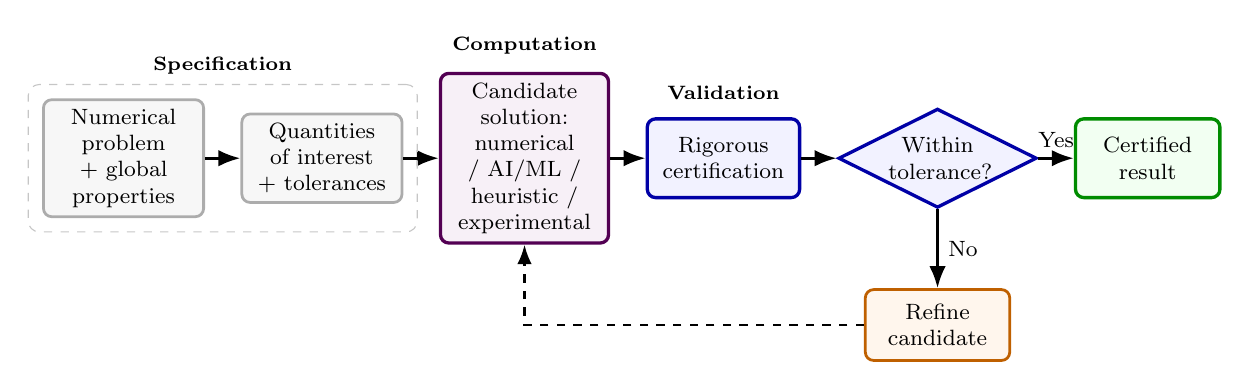
\begin{tikzpicture}[
        node distance=1.1cm and 0.45cm,
        >=Latex,
        every node/.style={font=\footnotesize, align=center},
        normal/.style={
            draw=gray!65,
            line width=1.0pt,
            rounded corners=3pt,
            fill=gray!6,
            minimum height=1.0cm,
            text width=1.8cm
        },
        computation/.style={
            draw=violet!65!black,
            line width=1.2pt,
            rounded corners=3pt,
            fill=violet!6,
            minimum height=1.0cm,
            text width=1.9cm
        },
        certification/.style={
            draw=blue!65!black,
            line width=1.2pt,
            rounded corners=3pt,
            fill=blue!5,
            minimum height=1.0cm,
            text width=1.7cm
        },
        success/.style={
            draw=green!55!black,
            line width=1.2pt,
            rounded corners=3pt,
            fill=green!5,
            minimum height=1.0cm,
            text width=1.6cm
        },
        retry/.style={
            draw=orange!75!black,
            line width=1.0pt,
            rounded corners=3pt,
            fill=orange!7,
            minimum height=0.9cm,
            text width=1.6cm
        },
        decision/.style={
            diamond,
            aspect=2,
            draw=blue!65!black,
            line width=1.2pt,
            fill=blue!5,
            inner sep=1pt,
            text width=1.25cm
        },
        flow/.style={->, line width=1.1pt},
        feedback/.style={->, line width=0.9pt, dashed}
    ]

    % Main nodes
    \node[normal] (problem)
        {Numerical problem\\+ global properties};

    \node[normal, right=of problem] (spec)
        {Quantities of interest\\+ tolerances};

    \node[computation, right=of spec] (candidate)
        {Candidate solution:\\numerical / AI/ML / heuristic / experimental};

    \node[certification, right=of candidate] (cert)
        {Rigorous\\certification};

    \node[decision, right=of cert] (test)
        {Within\\tolerance?};

    \node[success, right=of test] (result)
        {Certified result};

    \node[retry, below=1.0cm of test] (refine)
        {Refine candidate};

    % Main flow
    \draw[flow] (problem) -- (spec);
    \draw[flow] (spec) -- (candidate);
    \draw[flow] (candidate) -- (cert);
    \draw[flow] (cert) -- (test);
    \draw[flow] (test) -- node[above]{Yes} (result);
    \draw[flow] (test) -- node[right]{No} (refine);

    % Feedback loop
    \draw[feedback] (refine.west) -| (candidate.south);

    % Stage grouping
    \node[
        draw=gray!45,
        dashed,
        rounded corners=4pt,
        inner sep=5pt,
        fit=(problem)(spec),
        label={[font=\scriptsize\bfseries]above:Specification}
    ] {};

    \node[above=0.10cm of candidate, font=\scriptsize\bfseries]
        {Computation};

    \node[above=0.10cm of cert, font=\scriptsize\bfseries]
        {Validation};

    \end{tikzpicture}

    \caption{A proposed computational pipeline for exact numerics. The candidate
    solution may be produced by an approximate, heuristic, or experimental
    method. An independent certification stage determines whether the quantities
    of interest satisfy the required tolerances.}
    \label{fig:exact-numerics-pipeline}
\end{figure}

One could ask: if the method used to generate the candidate is largely irrelevant to the final guarantee, why not simply guess randomly until a candidate passes the validation test? The reason for retaining sophisticated, and potentially expensive, approximative solvers is that verification may itself be difficult to achieve. A good approximative method can produce candidates that are much more likely to admit tight and successful certification. Moreover, even when verification requires computational effort comparable to that of generating the approximate solution, in many applications this additional cost may be justified by the certainty provided by the final certification.

Such a synergy between computation and validation is particularly useful when the computational method is difficult to analyse directly. A powerful but uncontrolled method can be used to search for a good candidate, while the final guarantee is supplied independently. In this way, experimental methods can be made reliable and AI related results can be cured from hallucinations.
Systematic errors only slow down the process, but can't spoil the final certified result.
Therefore the output becomes suitable for use in subsequent calculations, mathematical arguments, or decision making.



\subsection{A few simple illustrative examples}

For some, it might still be a strange concept to give exact upper and lower bounds for a solution without knowing the precise solution. However, it is possible to give such bounds -- which are not necessarily the tightest possible, but nevertheless provide exact and true statements -- based only on an approximate solution and, typically, some global property of the problem. 

\subsubsection{A simple root guessing problem}

To demonstrate a basic exact-bound reasoning in the context of root finding, consider the following function and root-finding problem\footnote{Example (ix) in \cite{book:IntervalNeumaier1991}.}: 

\begin{equation} 
f(x) = x + \tanh(x), \qquad f(x) = 1. 
\end{equation} 

Let $x^*$ denote the exact solution. Let's imagine that we got a hint that the root is close to $x^\bullet=0.5$. Is there a way to say something exact about the accuracy of the guess without calculating the root? The answer is affirmative, because we can deduce a global property of the function $f$. 
It is easy to see that 

\begin{equation}
f'(x) = 1 + \operatorname{sech}^2(x) \in (1,2]. 
\end{equation} 

Therefore, using the mean value theorem \cite{book:Rudin}, we can make the following exact statement:

\begin{equation}
f(x^*)-f(x^\bullet) = f'(\xi)\,(x^*-x^\bullet), 
\end{equation} 

where $\xi$ lies between $x^\bullet$ and $x^*$. 
After taking the absolute value of both sides, we can state the following inequality: 

\begin{equation}
|f(x^*)-f(x^\bullet)| 
=
|f'(\xi)|\,|x^*-x^\bullet| 
\ge
\inf_{\xi \in \mathbb{R}} |f'(\xi)|\,|x^*-x^\bullet|. 
\end{equation} 

Since $\inf_{\xi \in \mathbb{R}} |f'(\xi)| = 1$ for this particular function, we obtain the following exact bound:

\begin{equation}
|x^*-x^\bullet| 
\le
\frac{|f(x^*)-f(x^\bullet)|} {\inf_{\xi \in \mathbb{R}} |f'(\xi)|} 
= 
|1-f(x^\bullet)| = |1-(0.5+\tanh(0.5))| 
\le 0.037883. 
\end{equation}

Therefore, with this educated (or lucky) guess, we can exactly state that 

\begin{equation}
x^* \in [0.462117,\,0.537883], \qquad \text{or equivalently} \qquad x^* = 0.5 \pm 0.037883. 
\end{equation}

\begin{figure}[H] 
\centering 
\begin{subfigure}[t]{0.4\textwidth} 
\centering 
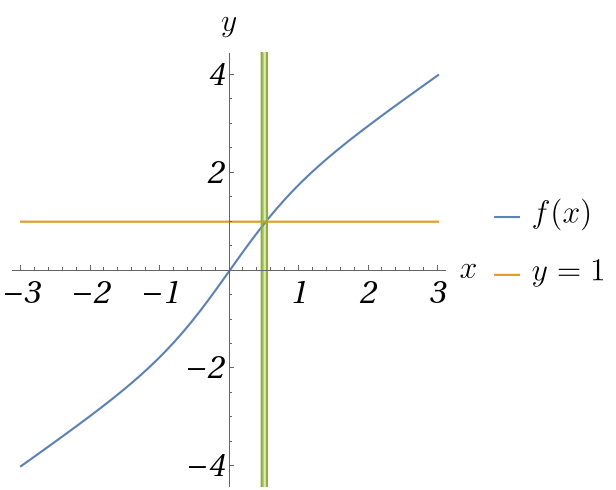
\includegraphics[width=\linewidth]{img/tanh01.png} 
\caption{Certified interval for $x^*$, $f(x^*)=1$, based on the approximate guess $x^\bullet=0.5$.}
\label{fig:tanh01} 
\end{subfigure} 
\hfill 
\begin{subfigure}[t]{0.48\textwidth} 
\centering 
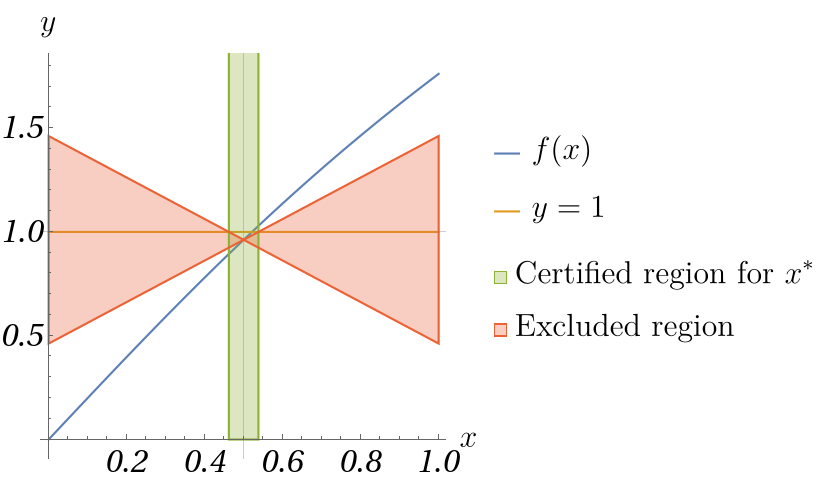
\includegraphics[width=\linewidth]{img/tanh02.png}
\caption{Closer view, showing the excluded region based on a global lower bound of the derivative of $f(x)$ (specifically $|f'(x)|\ge1$)} 
\label{fig:tanh02} 
\end{subfigure} 
\caption{Illustration of a simple ``a posteriori'' solution-certification example for $f(x)=x+\tanh(x)$. A good approximate guess $x^\bullet=0.5$, together with a global lower bound on $|f'(x)|$, gives a certified interval containing the exact solution $x^*$ for the equation $f(x^*)=1$.} 
\label{fig:tanh-root-certification} 
\end{figure}

\subsubsection{Newtons method with exact bounds}

Let say we have a $f \in C^2(\mathbb{R},\mathbb{R})$ (in fact it is enough to be twice differentiable (without the requirement of continuity\footnote{Or perhaps more generally that $f'(.)$ is a (locally) Lipschitz function.}), and boundedness of the second derivative on an open domain.)
And we search for a root of this function $x^* \in \mathbb{R}, \ f(x^*)= 0$.

If we can independently prove that on some open domain $\mathcal{D}$, containing a root ($x^* \in \mathcal{D}$) the absolute value of the second derivative is bounded:

\begin{equation}
    \exists M \in \mathbb{R}, \ \forall x \in \mathcal{D} \ |f''(x)|\le M
\end{equation}

Then -- if we are close enough to a root -- an exact interval can be determined:

Let say that we are at $x^\circ$, where the value is $f(x^\circ) \ne 0$ and we know the derivative $f'(x^\circ)$. By recalling Taylor's theorem \cite{book:Rudin}:

\begin{equation}
    f(x) = f(x^\circ) + f'(x^\circ) (x-x^\circ) + \frac{1}{2} f''(\xi) (x-x^\circ)^2, \quad \xi \in \{t\ x+ (1-t) \ x^\circ \ | \ t \in [0,1]]
\end{equation}

By assuming that $f(x)=0$ i.e. $x=x^*$ we have:

\begin{equation}
    |f(x^\circ) + f'(x^\circ) (x-x^\circ)| = \frac{1}{2} |f''(\xi)| (x-x^\circ)^2
\end{equation}

Excluded solution set

\begin{equation}
    \mathcal{E} = \{ x \in \mathbb{R} \ | \ |f(x^\circ) + f'(x^\circ) (x-x^\circ)| > \frac{1}{2} M (x-x^\circ)^2 \ \}
\end{equation}

The solution set can be defined as follows:

\begin{equation}
    \mathcal{S} : \text{Connected component of } \mathcal{E}^{\complement} = \mathbb{R} \setminus\mathcal{E} \ \text{including } x^{\bullet} = x^\circ - f(x^\circ)/f'(x^\circ)
\end{equation}


If

\begin{equation}
    \mathcal{S} \subseteq \mathcal{D} \implies \exists x^* \in \mathcal{S}, \ f(x^*)=0
\end{equation}

In the one dimensional case we can provide explicit lower and upper bounds from this observation simply by solving a second order inequality:

\begin{equation}
    |f(x^\circ) + f'(x^\circ) (x-x^\circ)| \le \frac{1}{2} M (x-x^\circ)^2
\end{equation}

For $2 M | f(x^\circ)|<f'(x^\circ)^2$

\begin{equation}
    I^\diamond
    =
    \left \{
    x^\circ - 
    \frac{f'(x^\circ)}{m} 
    \left ( 
    \sqrt{1-2 m \frac{f(x^\circ)}{f'(x^\circ)^2}}
    -
    1
    \right )
    \ {\Large |} \ 
    m \in [-M,0)\cup(0,M]
    \right \}
    \bigcup
    \left \{
    x^\circ - \frac{f(x^\circ)}{f'(x^\circ)}
    \right \}
\end{equation}

For $f(x^\circ)>0$ and $f'(x^\circ)>0$

\begin{equation}
    I^\diamond
    =
    \left [
    x^\circ - 
    \frac{f'(x^\circ)}{M} 
    \left ( 
    1-
    \sqrt{1-2 M \frac{f(x^\circ)}{f'(x^\circ)^2}}
    \right )
    ,
    x^\circ - 
    \frac{f'(x^\circ)}{M} 
    \left ( 
    \sqrt{1+2 M \frac{f(x^\circ)}{f'(x^\circ)^2}}
    -
    1
    \right )
    \right ]
\end{equation}

This reasonong essentially recovers the Newton-Kantorovich Theorem \cite{book:OrtegaIterativeSolutionOfNonlinearEquations}.

\paragraph{A note on determining the upper bound:}
In general determining a valid upper bound of the second derivative of a function on a domain $\mathcal{D}$ can be challenging. However there are a few simple techniques by which this can be done if the function $f(.)$ is constructed from simpler components.
If we define a symbolic algebra: $\mathcal{A}=<\mathbb{R},\cdot,\oplus,\mathsf{a}_1,\mathsf{a}_2,\dots>$, where atomic $\mathsf{a}_i$ corresponds to ``elementary functions'':

\begin{equation}
    \text{Eval}[\mathsf{a}_i](x) 
    =
    \phi_i(x)
\end{equation}

And for composite algebra elements $\mathsf{A} \in \mathcal{A}$ we define the evaluation as:

\begin{equation}
    \text{Eval}[c \cdot \mathsf{A}](x) 
    =
    c \cdot \text{Eval}[\mathsf{A}](x)
\end{equation}

\begin{equation}
    \text{Eval}[\mathsf{A}_1 \oplus \mathsf{A}_2](x)
    =
    \text{Eval}[\mathsf{A}_1](x) 
    +
    \text{Eval}[\mathsf{A}_2](x) 
\end{equation}

We can introduce an upper bound mapping for the second derivative from the algebra to the non-negative real numbers $\overline{\text{Max}}_2 : \mathcal{A} \mapsto \mathbb{R}_\ge$

\begin{equation}
    \overline{\text{Max}}_2[c \cdot \mathsf{A}] 
    =
    |c| \cdot \overline{\text{Max}}_2[\mathsf{A}] 
\end{equation}

\begin{equation}
    \overline{\text{Max}}_2[\mathsf{A}_1 \oplus \mathsf{A}_2]
    =
    \overline{\text{Max}}_2[\mathsf{A}_1] + \overline{\text{Max}}_2[\mathsf{A}_2]
\end{equation}

To enrich the algebra by multiplication $\mathcal{A}=<\mathbb{R},\cdot,\oplus,\otimes,\mathsf{a}_1,\mathsf{a}_2,\dots>$ we need to introduce the evaluation for the symbolic product:

\begin{equation}
    \text{Eval}[\mathsf{A}_1 \otimes \mathsf{A}_2](x)
    =
    \text{Eval}[\mathsf{A}_1](x) 
    \cdot
    \text{Eval}[\mathsf{A}_2](x) 
\end{equation}

and a similar concept to $\overline{\text{Max}}_2$ for the $n$-th derivative, $n\in\{0,1,2\}$.

\begin{equation}
    \overline{\text{Max}}_0[\mathsf{A}_1 \otimes \mathsf{A}_2] 
    =
    \overline{\text{Max}}_0[\mathsf{A}_1] \cdot \overline{\text{Max}}_0[\mathsf{A}_2]
\end{equation}

\begin{equation}
    \overline{\text{Max}}_1[\mathsf{A}_1 \otimes \mathsf{A}_2] 
    =
    \overline{\text{Max}}_1[\mathsf{A}_1] \cdot \overline{\text{Max}}_0[\mathsf{A}_2]
    +
    \overline{\text{Max}}_0[\mathsf{A}_1] \cdot \overline{\text{Max}}_1[\mathsf{A}_2]
\end{equation}

\begin{equation}
    \overline{\text{Max}}_2[\mathsf{A}_1 \otimes \mathsf{A}_2] 
    =
    \overline{\text{Max}}_2[\mathsf{A}_1] \cdot \overline{\text{Max}}_0[\mathsf{A}_2]
    +
    2 \cdot \overline{\text{Max}}_1[\mathsf{A}_1] \cdot \overline{\text{Max}}_1[\mathsf{A}_2]
    +
    \overline{\text{Max}}_0[\mathsf{A}_1] \cdot \overline{\text{Max}}_2[\mathsf{A}_2]
\end{equation}

Therefore if we have an algebra of function symbols $\mathcal{A}=<\mathbb{R},\cdot,\oplus,\otimes,\mathsf{a}_1,\mathsf{a}_2,\dots>$, where for all ``elementary'' $\mathsf{a}_i$ -- that corresponds to ``elementary functions'' $\phi_i(x) = \text{Eval}[\mathsf{a}_i](x)$ -- the $\overline{\text{Max}}_n[\mathsf{a}_i] \ge \sup_{x\in\mathcal{D}} \phi^{(n)}_i(x)$ are set, then for any composite function in the algebra the 
$\overline{\text{Max}}_2[.]$ value can be determined.

Generalization for any $n \in \mathbb{N}$:

\begin{equation}
    \overline{\text{Max}}_n[c \cdot \mathsf{A}] 
    =
    |c| \cdot \overline{\text{Max}}_n[\mathsf{A}] 
\end{equation}

\begin{equation}
    \overline{\text{Max}}_n[\mathsf{A}_1 \oplus \mathsf{A}_2]
    =
    \overline{\text{Max}}_n[\mathsf{A}_1] + \overline{\text{Max}}_n[\mathsf{A}_2]
\end{equation}

\begin{equation}
    \overline{\text{Max}}_n[\mathsf{A}_1 \otimes \mathsf{A}_2] 
    =
    \sum_{k=0}^n
    \binom{n}{k}
    \overline{\text{Max}}_k[\mathsf{A}_1] \cdot \overline{\text{Max}}_{n-k}[\mathsf{A}_2]
\end{equation}

\paragraph{Example:}
Let $\mathcal{D}=(-1,1)$

\begin{equation}
    f(x)=\exp(x)-\arctan(x)
\end{equation}

Therefore one possible symbolic representation is:

\begin{equation}
    \mathsf{A} = \mathsf{exp} \oplus ((-1) \cdot \mathsf{arctan})
    , \quad \text{Eval}[\mathsf{A}](x) = f(x)
\end{equation}

$\overline{\text{Max}}_2[\mathsf{exp}] = e$ and $\overline{\text{Max}}_2[\mathsf{arctan}] = 3/8 \sqrt{3}$, therefore:

\begin{equation}
    \overline{\text{Max}}_2[\mathsf{A}] = e +  3/8 \sqrt{3}
    \ge \sup_{x \in \mathcal{D}} |f''(x)|
\end{equation}

\subsubsection{Multi variate case}

The concept of exact solution sets are much more interesting in the multivariate case. (Because in one dimension for continuous problems it is often enough to find two points with opposite signs to guarantee a set containing a root.)

\href{https://en.wikipedia.org/wiki/Kantorovich_theorem}{Kantorovich theorem}

\section{Moderately powerful techniques}

We will demonstrate the simpler techniques on the quantum pendulum:

\begin{equation}
    H = -\frac{1}{2} \frac{\partial^2}{\partial\varphi^2} + g (1-\cos(\varphi))
\end{equation}

\subsection{Gershgorin circle}

(Geršgorin's circle)

\subsection{Brauer's ovals of Cassini}

\section{Quartic oscillator as a testing ground}

\begin{equation}
    H = \frac{1}{2} P^2+\frac{1}{2} \omega_0^2 \ X^2+\lambda \frac{1}{4!} X^4
\end{equation}

\begin{equation}
    H = \frac{1}{2} P^2+\frac{1}{2} \omega_0^2 \  X^2+g X^4
\end{equation}

\section{Controlled approximation}

\subsection{Majorization, minorization, envelope method}

Lemma:

\begin{equation}
    \forall x \in X, \ f(x) \ge g(x) 
    \implies
    \inf_{x \in X} f(x) \ge \inf_{x \in X} g(x)
\end{equation}

\begin{equation}
    \forall x \in X, \ f(x) \ge g(x) 
    \implies
    \sup_{x \in X} f(x) \ge \sup_{x \in X} g(x)
\end{equation}

Proof for inf:

\begin{equation}
    \forall x \in X, \ 
    f(x) \ge g(x) 
    \ge 
    \inf_{x \in X} g(x)
\end{equation}

Therefore $\inf_{x \in X} g(x)$ is a global lower bound for $f(.)$, so $\inf_{x\in X} f(x) \ge \inf_{x \in X} g(x)$

Lemma:

\begin{equation}
    \forall x \in X', \ f(x) \ge g(x), \ 
    X' \subseteq X
    \implies
    \inf_{x \in X'} f(x) \ge \inf_{x \in X} g(x)
\end{equation}

Proof for inf:

\begin{equation}
    \forall x \in X', \ 
    f(x) \ge g(x) 
    \ge 
    \inf_{x \in X'} g(x)
    \ge
    \inf_{x \in X} g(x)
\end{equation}

Therefore $\inf_{x \in X} g(x)$ is a global lower bound for $f(.)$, on $X'$, so $\inf_{x\in X'} f(x) \ge \inf_{x \in X} g(x)$.


For two self-adjoint linear operators $A$, $B$ on the finite $n$-dimensional vector complex vectorspace $V$ we have:

\begin{equation}
    A \succcurlyeq B
    \implies
    \lambda_i \ge \mu_i
\end{equation}

Proof:

\begin{equation}
    A \succcurlyeq B
    \iff
    \forall v \in V, \ v^* \cdot A \cdot v \ge v^* \cdot B \cdot v
\end{equation}

\begin{equation}
    \mu_1
    =
    \min_{v \in V, ||v||=1}
    v^* \cdot B \cdot v
    \le
    \min_{v \in V, ||v||=1}
    v^* \cdot A \cdot v
    =
    \lambda_1
\end{equation}

\begin{equation}
    \lambda_n
    =
    \max_{v \in V, ||v||=1}
    v^* \cdot A \cdot v
    \ge
    \max_{v \in V, ||v||=1}
    v^* \cdot B \cdot v
    =
    \mu_n
\end{equation}

\begin{equation}
    \lambda_k
    =
    \min_{V_k \subseteq V, \text{Dim}(V_k)=k} \max_{v\in V_k, ||v||=1} 
    v^* \cdot A \cdot v
\end{equation}

\begin{equation}
    \forall \  V_k\subseteq V  \max_{v\in V_k, ||v||=1} 
    v^* \cdot A \cdot v
    \ge
    \max_{v\in V_k, ||v||=1} 
    v^* \cdot B \cdot v
\end{equation}

Therefore 

\begin{equation}
        \lambda_k
    =
    \min_{V_k \subseteq V, \text{Dim}(V_k)=k} \max_{v\in V_k, ||v||=1} 
    v^* \cdot A \cdot v
    \ge
    \min_{V_k \subseteq V, \text{Dim}(V_k)=k} \max_{v\in V_k, ||v||=1} 
    v^* \cdot B \cdot v
    =
    \mu_k
\end{equation}

In case of linear operators on infinte dimensional separable Hilbert-spaces $\mathcal{H}$ if $A$ and $B$ are densly defined self-adjoint operators and both $A$ and $B$ have a point spectrum (at least for a finite low lying eigenvalues) -- technically both operators having a countable set of eigenvalues and eigenvectors below their ``essential spectrum'' --  and their spectrum is bounded from below, then

\begin{equation}
    A \succcurlyeq B
    \implies
    \lambda_k \ge \mu_k
\end{equation}

Proof:

\begin{equation}
    A \succcurlyeq B
    \iff
    \forall \psi \in \mathcal{Q}(A) \cap \mathcal{Q}(B), \ 
    \langle \psi | A | \psi \rangle
    \ge
    \langle \psi | B | \psi \rangle
\end{equation}

Where $\mathcal{Q}(A) \subseteq \mathcal{H}$ stands for the linear space, where the quadratic form is defined, i.e. $\langle \psi | A | \psi \rangle \in \mathbb{R}$.

In fact in this case -- when both $A$ and $B$ are bounded from below and $A \succcurlyeq B$ -- $\mathcal{Q}(A) \subseteq \mathcal{Q}(B)$ because for a state $\psi \in \mathcal{Q}(A)$ the quadretic form $\langle \psi | A | \psi \rangle$ is defined, then $\langle \psi | B | \psi \rangle$ has to be finite and defined as well. This implies that $\mathcal{Q}(A) \cap \mathcal{Q}(B) = \mathcal{Q}(A)$ that is a dense subspace of $\mathcal{H}$.

Utiliying the Min-max theorem (in \href{https://www.mat.univie.ac.at/~gerald/ftp/book-schroe/schroe.pdf}{Theorem 4.10})

\begin{equation}
    \lambda_k
    =
    \inf_{\mathcal{H}_k \subseteq \mathcal{H}, \text{Dim}(\mathcal{H}_k)=k} \sup_{\psi\in \mathcal{H}_k, ||\psi||=1} 
    \langle \psi |  A | \psi \rangle
\end{equation}

\begin{equation}
    \forall \  \mathcal{H}_k\subseteq \mathcal{Q}(A)
    \sup_{\psi\in \mathcal{H}_k, ||\psi||=1} 
    \langle \psi |  A | \psi \rangle
    \ge
    \sup_{\psi\in \mathcal{H}_k, ||\psi||=1} 
    \langle \psi |  B | \psi \rangle
    \end{equation}

Therefore:

\begin{equation}
    \lambda_k
    =
    \inf_{\mathcal{H}_k \subseteq \mathcal{Q}(A), \text{Dim}(\mathcal{H}_k)=k} \sup_{\psi\in \mathcal{H}_k, ||\psi||=1} 
    \langle \psi |  A | \psi \rangle
    \ge
    \inf_{\mathcal{H}_k \subseteq \mathcal{Q}(B), \text{Dim}(\mathcal{H}_k)=k} \sup_{\psi\in \mathcal{H}_k, ||\psi||=1} 
    \langle \psi |  B | \psi \rangle
    =
    \mu_k
\end{equation}

In particular we will show that how envelope theory \cite{arxiv:EnvelopeTheory} can be narrated as a minorzation - majorization technique.

\subsubsection{Quadratic potential}

\begin{equation}
    H = \frac{1}{2} P^2+X^4
\end{equation}

\begin{equation}
    \check{H}(a) =  \frac{1}{2} P^2+a^4+2 a^2(X-a)(X+a)
\end{equation}

\begin{equation}
    \check{H}(a) =  \frac{1}{2} P^2+\frac{1}{2} 4 a^2 X^2 - 2 a^4
\end{equation}

\begin{equation}
    \check{E}_n(a) = 2 a (n + 1/2) - 2 a^4 
\end{equation}

\begin{equation}
    \check{E}^*_n = \sup_{a>0} \ \check{E}_n(a)
\end{equation}

\begin{equation}
    \check{E}^*_n = \frac{3}{8} (1 + 2 n)^{4/3}, \quad
    a^*_n=\frac{1}{2} (1 + 2 n)^{1/3}
\end{equation}

\begin{equation}
    E_n \ge \check{E}^*_n = \frac{3}{8} (1 + 2 n)^{4/3}
\end{equation}

\subsubsection{Rectangular potential wells}

One of the simplest quantummechanical system is a particle in a ptential well, with infinite wall.

\begin{equation}
    V(x;V_0,a) =
    \begin{cases}
        V_0 & \text{if } -a < x < a \\
        \infty & \text{otherwise}
    \end{cases}
\end{equation}

This definition is ofcourse far from being precise -- and this operator is not densly defined on squqre integrable functions on the whole numberline $L^2(\mathbb{R},\mathbb{C})$ --, but it can be defined as a limiting case of densly defined operators.

\begin{equation}
    V(x;V_0,a;\Lambda) =
    \begin{cases}
        V_0 & \text{if } -a < x < a \\
        \Lambda \  V_{\text{ext}}(x) & \text{otherwise}
    \end{cases}
\end{equation}

Where $V_\text{ext}(.)$ is a positive continuous function with positive global lower bound $\inf_{x \in \mathbb{R}} V_\text{ext}(x) > 0$. If we wish to keep for instance the Schwartz functions on the whole number line to belong to the domain of $V(x;V_0,a;\Lambda)$ for any finite $\Lambda>0$, then we can demand that $V_\text{ext}(x)$ has at most polynomial growth as $|x|$ goes to infinity.
Quantities related to $V(x;V_0,a)$ can then be understood as the $\Lambda \to \infty$ limiting cases of expressions including the regularized $V(x;V_0,a;\Lambda)$ potential.

\begin{equation}
    \psi_n(x)=\frac{1}{\sqrt{a}}\sin(k_n (x+a)), \quad
    E_n = \frac{1}{2} k_n^2 + V_0
\end{equation}

\begin{equation}
    k_n=\pi \frac{n+1}{2 a}
\end{equation}

\subsubsection{Pöschl–Teller potential}

\subsection{Krylov-Weinstein bound}

For a self adjoint $A$ 

\begin{equation}
    \exists v \in V \setminus \{\underline{0}\} , \varepsilon \ge 0 ,  \ v^* \cdot (A-\alpha)^2 \cdot v \le \varepsilon \ v^* \cdot v
    \implies
    \exists \lambda_i, \ |\lambda_i-\alpha| \le \sqrt{\varepsilon}
\end{equation}

Proof

\begin{equation}
    \forall v \in V, \  v^* \cdot (A-\alpha)^2 \cdot v  \ge \min_{i} (\lambda_i-\alpha)^2 \ v^* \cdot v
\end{equation}

\begin{equation}
    \exists v \in V \setminus \{\underline{0}\} , \varepsilon \ge 0 ,  \ v^* \cdot (A-\alpha)^2 \cdot v \le \varepsilon \ v^* \cdot v
    \implies
    \varepsilon \ge  \min_{i} (\lambda_i-\alpha)^2
\end{equation}

\begin{equation}
    \min_{i} (\lambda_i-\alpha)^2 \le \varepsilon
    \implies
    \exists \lambda_i, \ |\lambda_i-\alpha| \le \sqrt{\varepsilon}
\end{equation}

Excluding eigenvalues:

\begin{equation}
    \exists \varepsilon \ge 0 , \ 
    (A-\alpha)^2 \succcurlyeq \varepsilon
    \implies
    \nexists \ \lambda_i, \ \lambda_i \in [\alpha-\sqrt{\varepsilon},\alpha+\sqrt{\varepsilon}]
\end{equation}

Proof

Lets assume that for some $\varepsilon>0$ there is an eigenvalue $\lambda_i \in [\alpha-\sqrt{\varepsilon},\alpha+\sqrt{\varepsilon}]$. Then there is an eigenvector $v_i \in V \setminus \{\underline{0}\}$ such that $A\cdot v_i=\lambda_i v_i$.
Then $(A-\alpha)^2\cdot v_i = (\lambda_i-\alpha)^2 v_i$ and

\begin{equation}
    \frac{v^*_i \cdot (A-\alpha)^2 \cdot v_i}{v^*_i \cdot v_i} = (\lambda_i-\alpha)^2 \le \epsilon
\end{equation}

Bur from

\begin{equation}
    (A-\alpha)^2 \succcurlyeq \varepsilon
    \implies
    \forall v \in V \setminus \{\underline{0}\} , \ 
    \frac{v^*_i \cdot (A-\alpha)^2 \cdot v_i}{v^*_i \cdot v_i} 
    \ge 
    \varepsilon
\end{equation}

Which is a contradiction.


\begin{equation}
    H = \frac{1}{2} P^2 + V(X)
\end{equation}

\begin{equation}
    (H-E)^2 = \frac{1}{4} P^4 + \frac{1}{2}(P^2 \ (V(X)-E)+ (V(X)-E) \ P^2) + (V(X)-E)^2
\end{equation}

\begin{equation}
    [V(X),P] = i V'(X)
\end{equation}

\begin{equation}
    (H-E)^2 = \frac{1}{4} P^4 + P \ (V(X)-E) \  P + [[V(X)-E,P],P] + (V(X)-E)^2
\end{equation}

\begin{equation}
    (H-E)^2 = \frac{1}{4} P^4 + P \ (V(X)-E) \  P - V''(X) + (V(X)-E)^2
\end{equation}

Minorization:

We can introduce a peacewise constant, minorizing potential $\check{V}(x;E)$, $\forall x \in \mathbb{R}, \ \check{V}(x;E) \le V(x)-E$ and a minorization square-like potential $\check{W}(X;E)$ 
$\forall x \in \mathbb{R}, \ \check{W}(x;E) \le  (V(x)-E)^2 - V''(x)$

\begin{equation}
    \left ( \frac{1}{4} P^2 + P \ \check{V} \ P + \check{W} \right ) \psi(x) = \varepsilon \  \psi(x)
\end{equation}

With the ansatz $\psi(x) = e^{ik \ x} $

\begin{equation}
    \frac{1}{4}k^4 - \check{V} k^2 + \check{W} = \varepsilon
\end{equation}

This has four soultions:

\begin{equation}
    k_{s_1,s_2} = s_1\sqrt{2} \sqrt{s_2 \sqrt{\check{V}^2 - \check{W} + \varepsilon} + \check{V}}
\end{equation}

\begin{equation}
    \psi(x) = A_{++} e^{ik_{++} x} + A_{+-} e^{ik_{+-} x} + A_{-+} e^{ik_{-+} x} + A_{--} e^{ik_{--} x}
\end{equation}

With $A_{++}, A_{+-}, A_{-+}, A_{--} \in \mathbb{C}$

\begin{equation}
    (H-E)^2 = \frac{1}{4} P^4 + (V(X)-E) \  P^2 - [V(X)-E,P] P - V''(X) + (V(X)-E)^2
\end{equation}

\begin{equation}
    (H-E)^2 = \frac{1}{4} P^4 + (V(X)-E) \  P^2 - iV'(X) P - V''(X) + (V(X)-E)^2
\end{equation}

For piecwise constant V(x), going from $V_{-}$ for $x<0$ and $V_{+}$ for $x>0$

\begin{equation}
    (H-E)^2 \psi(x) = \frac{1}{4} \psi''''(x) + (V(x)-E) (-\psi''(x)) - i (V_{+}-V_{-}) \delta(x) (-i \psi'(x)) - V''(X) \psi(x) + (V(X)-E)^2 \psi(x)
\end{equation}

\begin{equation}
    (H-E)^2 \psi(x) = 
    \varepsilon \ \psi(x)
\end{equation}

\begin{equation}
    \int_{-\Delta}^\Delta (H-E)^2 \psi(x) \ dx
    =
    \int_{-\Delta}^\Delta \varepsilon \ \psi(x) \ dx
\end{equation}

\begin{equation}
    \lim_{\Delta \to 0^+}\int_{-\Delta}^\Delta \psi''''(x) \ dx
    =
    \psi'''_+ - \psi'''_-
\end{equation}

\begin{equation}
    \lim_{\Delta \to 0^+}\int_{-\Delta}^\Delta (V(x)-E) (-\psi''(x)) \ dx
    =
    \lim_{\Delta \to 0^+}
    [(V(x)-E)(-\psi'(x))]_{-\Delta}^\Delta
    -
    \int_{-\Delta}^\Delta V'(x) (-\psi'(x)) \ dx
\end{equation}

$0$ if $\psi'_+=\psi'_-$

\begin{equation}
    \lim_{\Delta \to 0^+}\int_{-\Delta}^\Delta (V_{+}-V_{-}) \delta(x)  \psi'(x) \ dx
    =
    (V_{+}-V_{-}) \psi'(0)
\end{equation}

As $\Delta \to 0^+$ we get:

\begin{equation}
    \frac{1}{4} (\psi'''_+ - \psi'''_-) 
    + 
    (V_{+}-V_{-}) \psi'(0)
    =
    0
\end{equation}

\begin{equation}
    \psi_{-}=\psi_{+}=\psi(0), \quad
    \psi'_{-}=\psi'_{+}=\psi'(0), \quad
    \psi''_{-}=\psi''_{+}=\psi''(0), \quad
\end{equation}

\subsubsection{Auxiliary space methods}

If we have a selfadjoint Hamiltonian operator $H$ on a Hilbert space $\mathcal{H}$, then we can try to find an $F$ operator on an extended Hilbert space $\mathcal{H} \otimes V$ that $F^2$ is ``close to'' $H \otimes I$.

\begin{equation}
    H=P^2+X^4
\end{equation}

\begin{equation}
    F=P\otimes \sigma_x + W(X) \otimes \sigma_y
\end{equation}

\begin{equation}
    F^2 = P^2 \otimes I + W(X)^2 \otimes I + P W(x) \otimes \sigma_x \sigma_y + W(X) P \otimes \sigma_y \sigma_x
\end{equation}

\begin{equation}
    F^2 = P^2 \otimes I + W(X)^2 \otimes I - i [P, W(x)] \otimes \sigma_z
\end{equation}

\begin{equation}
    F^2 = P^2 \otimes I + W(X)^2 \otimes I - W'(X) \otimes \sigma_z
\end{equation}

If we chose $W(X)=X^2$, then we get:

\begin{equation}
    F^2 = P^2 \otimes I +X^4 \otimes I - 2 X \otimes \sigma_z
\end{equation}

This is not exactly the quartic potential we had in the original $H$, but the $- 2 X \otimes \sigma_z$ is ``small'' relative to the $P^2 \otimes I +X^4 \otimes I$.

This means that the $x^4 \pm 2x$ potential can be minorized and majorized by $g (x-x_0)^4+v_0$ potentials, therefore knowing the eigenvalues for the potential $x^4 \pm 2x$ can provide finite upper and lower bounds for the pure quartic potential.

Using the Krylov-Weinstein bound for $F$:

Lemma:
If we have a self adjoint $A$

\begin{equation}
    v^* \cdot (A-\sqrt{E})^2 \cdot v \le \varepsilon \ v^* \cdot v
\end{equation}

then there is a $\lambda$ eigenvalue of $A^2$ that:

\begin{equation}
    \exists \lambda, |\lambda-E|\le \sqrt{\varepsilon} (2\sqrt{E}+\sqrt{\varepsilon})
\end{equation}

Proof

\begin{equation}
    v^* \cdot (A-\sqrt{E})^2 \cdot v = \varepsilon \ v^* \cdot v
    \implies
    \exists \mu, \ (\mu-\sqrt{E})^2 \le \varepsilon
\end{equation}

\begin{equation}
    |\lambda - E| = |\mu-\sqrt{E}| \  | \mu + \sqrt{E}|
\end{equation}

\begin{equation}
    | \mu + \sqrt{E}| = | \mu - \sqrt{E} + 2 \sqrt{E}| \le | \mu - \sqrt{E}| + 2 \sqrt{E}
\end{equation}

\begin{equation}
    |\lambda - E| \le \sqrt{\varepsilon} (2 \sqrt{E} + \sqrt{\varepsilon})
\end{equation}

\begin{equation}
    (F-\sqrt{E})^2 = F^2 + E - 2 \sqrt{E} \  F
\end{equation}

\begin{equation}
    (F-\sqrt{E})^2 =
    \begin{bmatrix}
        P^2 + W(X)^2 - W'(X) + E & 2 \sqrt{E} (P+i W(X)) \\
        2 \sqrt{E} (P-i W(X)) & P^2 + W(X)^2 + W'(X) + E
    \end{bmatrix}
\end{equation}

And whenever we can find a pair of functions $\psi_\uparrow(x),\psi_\downarrow(x)$ that 

\begin{equation}
    [\psi_\uparrow^*(x),\psi_\downarrow^*(x)] 
    \begin{bmatrix}
        P^2 + W(X)^2 - W'(X) + E & 2 \sqrt{E} (P+i W(X)) \\
        2 \sqrt{E} (P-i W(X)) & P^2 + W(X)^2 + W'(X) + E
    \end{bmatrix}
    \begin{bmatrix}
        \psi_\uparrow(x) \\
        \psi_\downarrow(x)
    \end{bmatrix}
    =
    \varepsilon
\end{equation}

then we know that ...

In the quartic case the $x \to -x$ is a symmetry, therefore we can look for the $(\psi_\uparrow(x),\psi_\downarrow(x))$ pairs as $(\psi(x)/\sqrt{2},\psi(-x)/\sqrt{2})$

\subsubsection{Super symmetric field theory example}

The auxiliary space method can be generalized to SUSY field theories, where observable operators -- such as H and P -- can be defined as the products of some charge operators $\mathcal{Q}$. In the following we present a sketch, how non-trivial approximative dispersion relations can be derived in 1+1D SUSY field theories.

{\bf ChatGPT assisted:}

\paragraph{Basic construction: interacting \(1+1\)D supersymmetric QFT with (real) superpotential $W$}

We consider the standard \(1+1\)-dimensional \(\mathcal N=(1,1)\) Wess--Zumino model with one real scalar field \(\phi(t,x)\) and one Majorana fermion $\psi_\pm(t,x)$, written in terms of two real chiral components
\[
\psi_+(t,x), \qquad \psi_-(t,x).
\]
We use Minkowski coordinates $x^\mu$ and metric $\eta_{\mu \nu}$
\[
    x^0=t, \quad x^1=x, \quad 
    \eta=\begin{bmatrix}
    1 & 0 \\ 0 & -1 \end{bmatrix},
\]
and abbreviate
\[
\dot\phi=\partial_t\phi(t,x), \qquad \phi'=\partial_x\phi(t,x).
\]

\paragraph{Lagrangian density}

Given a real superpotential \(W(\phi)\), the component Lagrangian density is
\begin{equation}
\boxed{
\mathcal{L}
=
\frac12 \dot\phi^{\,2}
-\frac12 \phi'^{\,2}
+\frac{i}{2}\psi_+(\partial_t-\partial_x)\psi_+
+\frac{i}{2}\psi_-(\partial_t+\partial_x)\psi_-
-\frac12 \bigl(W'(\phi)\bigr)^2
- W''(\phi)\,\psi_+\psi_- .
}
\end{equation}

The bosonic potential is therefore
\begin{equation}
\boxed{
V(\phi)=\frac12 \bigl(W'(\phi)\bigr)^2.
}
\end{equation}

This defines an interacting QFT whenever \(W\) is nonlinear.

\paragraph{Canonical momentum}

The conjugate momentum of \(\phi\) is
\begin{equation}
\boxed{
\pi(t,x)=\frac{\partial \mathcal L}{\partial \dot\phi}=\dot\phi.
}
\end{equation}

\paragraph{Hamiltonian density and Hamiltonian}

The Hamiltonian density is
\begin{equation}
\boxed{
\mathcal H
=
\frac12 \pi^2
+\frac12 \phi'^2
+\frac12 \bigl(W'(\phi)\bigr)^2
-\frac{i}{2}\psi_+\partial_x\psi_+
+\frac{i}{2}\psi_-\partial_x\psi_-
+W''(\phi)\,\psi_+\psi_- .
}
\end{equation}
Hence the Hamiltonian is
\begin{equation}
\boxed{
H=\int dx\,\mathcal H.
}
\end{equation}

\paragraph{Momentum density and momentum}

The momentum density is
\begin{equation}
\boxed{
\mathcal P
=
\pi\,\phi'
-\frac{i}{2}\psi_+\partial_x\psi_+
-\frac{i}{2}\psi_-\partial_x\psi_- .
}
\end{equation}
Hence the spatial momentum operator is
\begin{equation}
\boxed{
P=\int dx\,\mathcal P.
}
\end{equation}

\paragraph{Equal-time canonical brackets}

At equal time, the canonical relations are
\begin{equation}
\boxed{
[\phi(x),\pi(y)]=i\delta(x-y),
}
\end{equation}
and
\begin{equation}
\boxed{
\{\psi_+(x),\psi_+(y)\}=\delta(x-y), \qquad
\{\psi_-(x),\psi_-(y)\}=\delta(x-y), \qquad
\{\psi_+(x),\psi_-(y)\}=0.
}
\end{equation}

\paragraph{Self-adjointness of the fields}

\[
\phi^\dagger=\phi,
\qquad
\psi_+^\dagger=\psi_+,
\qquad
\psi_-^\dagger=\psi_-.
\]

Thus \(\phi\) is a real scalar field, while \(\psi_\pm\) are real Majorana fermion components.  
In particular, for a real superpotential \(W(\phi)\),
\[
W(\phi)^\dagger=W(\phi),
\qquad
W'(\phi)^\dagger=W'(\phi).
\]

\paragraph{Supercharges}

A convenient Hermitian choice of supercharges is
\begin{equation}
\boxed{
Q_+
=
\int dx\,
\Big[
(\pi+\phi')\psi_+
-
W'(\phi)\psi_-
\Big]
=
Q_+^\dagger
}
\end{equation}
\begin{equation}
\boxed{
Q_-
=
\int dx\,
\Big[
(\pi-\phi')\psi_-
+
W'(\phi)\psi_+
\Big]
=
Q_-^\dagger
}
\end{equation}

\paragraph{Supersymmetry algebra}

These satisfy the \(1+1\)-dimensional supersymmetry algebra
\begin{equation}
\boxed{
\{Q_+,Q_+\}=2(H+P), \qquad
\{Q_-,Q_-\}=2(H-P), \qquad
\{Q_+,Q_-\}=2Z.
}
\end{equation}
Here
\begin{equation}
\boxed{
Z=\int dx\,\partial_x W(\phi)
=
W(\phi(+\infty))-W(\phi(-\infty))
}
\end{equation}
is the topological central charge on the line.

On a spatial circle, or in the topologically trivial sector, one usually has $Z=0$.

From the first two anti-commutators we have:

\begin{equation}
\boxed{
Q_+^2=H+P, \qquad Q_-^2=H-P.
}
\end{equation}

\paragraph{Dispersion relation}

If \(|\Psi\rangle\) is a simultaneous eigenstate of energy and momentum,
\begin{equation}
H|\Psi\rangle=E|\Psi\rangle, \qquad P|\Psi\rangle=p|\Psi\rangle,
\end{equation}
then in the sector \(Z=0\),
\begin{equation}
\boxed{
Q_+^2|\Psi\rangle=(E+p)|\Psi\rangle, \qquad
Q_-^2|\Psi\rangle=(E-p)|\Psi\rangle.
}
\end{equation}
Thus it is natural to define the chiral energies
\begin{equation}
\boxed{
E_+=E+p, \qquad E_-=E-p,
}
\end{equation}
so that
\begin{equation}
\boxed{
E=\frac{E_++E_-}{2}, \qquad p=\frac{E_+-E_-}{2}.
}
\end{equation}

This is the basic reason why the dispersion relation can be studied through the supercharges \(Q_\pm\).

\paragraph{Complex supercharge.}
Define the complex combination
\begin{equation}
\boxed{
\mathcal Q := Q_+ + i Q_-,
\qquad
\mathcal Q^\dagger = Q_+ - i Q_-.
}
\end{equation}
A direct computation gives
\begin{equation}
\boxed{
\mathcal Q^2
=
(Q_+ + iQ_-)^2
=
Q_+^2 - Q_-^2 + i\{Q_+,Q_-\}
=
2P + 2iZ,
}
\end{equation}
and similarly
\begin{equation}
\boxed{
(\mathcal Q^\dagger)^2 = 2P - 2iZ.
}
\end{equation}
Moreover,
\begin{equation}
\boxed{
\{\mathcal Q,\mathcal Q^\dagger\}
=
2(Q_+^2+Q_-^2)
=
4H.
}
\end{equation}
The ordinary commutator is
\begin{equation}
\boxed{
[\mathcal Q,\mathcal Q^\dagger]
=
-2i[Q_+,Q_-],
}
\end{equation}
so \(\mathcal Q\) is not normal in general.

\paragraph{Rest frame and topologically trivial sector.}
In the sector
\[
P=0,\qquad Z=0,
\]
one has
\begin{equation}
\boxed{
\mathcal Q^2=0,
\qquad
\{\mathcal Q,\mathcal Q^\dagger\}=4H.
}
\end{equation}
Thus \(\mathcal Q\) is nilpotent in the rest frame, and the Hamiltonian is recovered from the anticommutator:
\begin{equation}
\boxed{
H=\frac14\bigl(\mathcal Q\mathcal Q^\dagger+\mathcal Q^\dagger\mathcal Q\bigr).
}
\end{equation}

\paragraph{Important remark.}
Since \(\mathcal Q^2=0\) in the sector \(P=Z=0\), every exact eigenvalue of \(\mathcal Q\) is zero. Therefore an ``approximate eigenvector'' of \(\mathcal Q\) alone cannot determine a positive rest mass: it can only test closeness to the kernel of \(\mathcal Q\), i.e. to a supersymmetric ground state.

To obtain a positive rest-mass bound for an excited bound state, one should instead use the auxiliary self-adjoint operator
\begin{equation}
\boxed{
\mathbb D :=
\begin{pmatrix}
0 & \mathcal Q^\dagger\\
\mathcal Q & 0
\end{pmatrix}
}
\qquad
\text{on }\mathcal H\otimes \mathbb C^2.
\end{equation}
Then \(\mathbb D^\dagger=\mathbb D\), and in the sector \(P=Z=0\),
\begin{equation}
\boxed{
\mathbb D^2
=
\begin{pmatrix}
\mathcal Q^\dagger\mathcal Q & 0\\
0 & \mathcal Q\mathcal Q^\dagger
\end{pmatrix}.
}
\end{equation}
Using
\[
\mathcal Q^\dagger\mathcal Q+\mathcal Q\mathcal Q^\dagger=4H,
\]
one sees that \(\mathbb D\) is the natural square-root object for the rest-frame problem.

\paragraph{Trial state.}
Let \(\Psi^\bullet\in\mathcal H\) be a normalized trial state representing a candidate \(P=0\) bound state, and form the doubled-space trial vector
\begin{equation}
\boxed{
\Phi^\bullet :=
\begin{pmatrix}
\Psi^\bullet\\
\Psi^\bullet
\end{pmatrix}
\in \mathcal H\otimes \mathbb C^2.
}
\end{equation}

\paragraph{Approximate \(\mathbb D\)-eigenvector and Krylov--Weinstein bound.}
Assume that for some \(d\ge 0\),
\begin{equation}
\boxed{
\|(\mathbb D-d)\Phi^\bullet\|^2 \le \varepsilon.
}
\end{equation}
Since \(\mathbb D\) is self-adjoint, the spectral theorem implies that there exists
\[
\mu\in \operatorname{spec}(\mathbb D)
\]
such that
\begin{equation}
|\mu-d|\le \sqrt{\varepsilon}.
\end{equation}
Squaring,
\[
\lambda:=\mu^2\in \operatorname{spec}(\mathbb D^2),
\]
and therefore
\begin{equation}
\boxed{
|\lambda-d^2|
\le
\sqrt{\varepsilon}\,\bigl(2d+\sqrt{\varepsilon}\bigr).
}
\end{equation}

\paragraph{From \(\mathbb D^2\) to the rest mass.}
In the rest frame, a stable bound state of mass \(M\) satisfies
\[
H\Psi = M\Psi.
\]
Since \(\mathbb D^2\) has diagonal blocks \(\mathcal Q^\dagger\mathcal Q\) and \(\mathcal Q\mathcal Q^\dagger\), and
\[
\mathcal Q^\dagger\mathcal Q+\mathcal Q\mathcal Q^\dagger=4H,
\]
the spectrum of \(\mathbb D^2\) is controlled by the rest-energy spectrum. In particular, if \(\Phi^\bullet\) has good overlap with one rest-frame bound-state multiplet, then the corresponding mass \(M\) satisfies the estimate
\begin{equation}
\boxed{
|\,4M - d^2\,|
\;\lesssim\;
\sqrt{\varepsilon}\,\bigl(2d+\sqrt{\varepsilon}\bigr),
}
\end{equation}
or equivalently
\begin{equation}
\boxed{
\left|\,M-\frac{d^2}{4}\,\right|
\;\lesssim\;
\frac14\,\sqrt{\varepsilon}\,\bigl(2d+\sqrt{\varepsilon}\bigr).
}
\end{equation}
Thus the rest mass is approximated by
\begin{equation}
\boxed{
M \approx \frac{d^2}{4},
}
\end{equation}
with an error controlled by the residual \(\varepsilon\).

\paragraph{Conclusion.}
The complex supercharge \(\mathcal Q\) is the natural nilpotent object in the rest-frame sector \(P=Z=0\), but by itself it only probes the supersymmetric kernel. For a positive rest-mass estimate one should pass to the auxiliary self-adjoint operator \(\mathbb D\). If \(\Phi^\bullet\) is an approximate \(\mathbb D\)-eigenvector, then a Krylov--Weinstein bound yields a quantitative estimate for the rest mass of the bound state. Once the rest mass \(M\) of a stable bound state is known, Lorentz invariance fixes the full dispersion relation:
\begin{equation}
\boxed{
E(p)=\sqrt{p^2+M^2}.
}
\end{equation}

\paragraph{Two simple interacting choices of superpotential}

A convenient class of \(1+1\)-dimensional \(\mathcal N=(1,1)\) supersymmetric field theories is obtained by choosing a real superpotential \(W(\phi)\). Two simple and useful interacting examples are the following.

\paragraph{1. Quartic Wess--Zumino model.}
Take
\begin{equation}
\boxed{
W(\phi)=\frac{m}{2}\phi^2+\frac{g}{4}\phi^4.
}
\end{equation}
Then
\begin{equation}
W'(\phi)=m\phi+g\phi^3,
\qquad
W''(\phi)=m+3g\phi^2.
\end{equation}
This model reduces to the free massive theory when \(g=0\), and becomes interacting for \(g\neq 0\). Around the vacuum at \(\phi=0\), the tree-level mass is \(m\), while the exact physical one-particle mass is expected to depend nontrivially on the coupling \(g\).

\paragraph{2. Supersymmetric sine-Gordon model.}
Take
\begin{equation}
\boxed{
W(\phi)=\frac{\mu}{\beta^2}\cos(\beta\phi).
}
\end{equation}
Then
\begin{equation}
W'(\phi)=-\frac{\mu}{\beta}\sin(\beta\phi),
\qquad
W''(\phi)=-\mu\cos(\beta\phi).
\end{equation}
This is a genuinely interacting model with a periodic vacuum structure. The parameter \(\beta\) controls the interaction strength, and the physical spectrum is expected to depend nontrivially on \(\beta\). It is a natural candidate for studying nontrivial one-particle states, bound states, and topological sectors.

\paragraph{Summary.}
The quartic Wess--Zumino model is a simple deformation of the free massive theory and is a natural first testing ground. The supersymmetric sine-Gordon model is more structurally rich and is a natural target for studying genuinely nontrivial interacting supersymmetric spectra.



\subsection*{Quartic Wess--Zumino model at rest: explicit \(\mathcal Q\), \(\mathbb D\), and trial state}

Consider the \(1+1\)-dimensional \(\mathcal N=(1,1)\) Wess--Zumino model with
\begin{equation}
\boxed{
W(\phi)=\frac{m}{2}\phi^2+\frac{g}{4}\phi^4.
}
\end{equation}
Then
\begin{equation}
W'(\phi)=m\phi+g\phi^3,
\qquad
W''(\phi)=m+3g\phi^2.
\end{equation}

We work in the topologically trivial sector \(Z=0\), and in the rest-frame sector \(P=0\).

\paragraph{Real supercharges.}
A standard choice of supercharges is
\begin{equation}
\boxed{
Q_+
=
\int_0^L dx\,
\Big[(\pi+\phi')\psi_+-(m\phi+g\phi^3)\psi_-\Big],
}
\end{equation}
\begin{equation}
\boxed{
Q_-
=
\int_0^L dx\,
\Big[(\pi-\phi')\psi_-+(m\phi+g\phi^3)\psi_+\Big].
}
\end{equation}

\paragraph{Complex supercharge.}
Define
\begin{equation}
\boxed{
\mathcal Q:=Q_+ + iQ_-,
\qquad
\mathcal Q^\dagger = Q_+ - iQ_-.
}
\end{equation}
Substituting the explicit formulas for \(Q_\pm\),
\begin{equation}
\boxed{
\mathcal Q
=
\int_0^L dx\,
\Big[
(\pi+\phi')\psi_+
+i(\pi-\phi')\psi_-
+(m\phi+g\phi^3)(\,i\psi_+ - \psi_-)
\Big].
}
\end{equation}
It is convenient to split
\begin{equation}
\mathcal Q=\mathcal Q^{(0)}+g\,\Delta\mathcal Q,
\end{equation}
with
\begin{equation}
\boxed{
\mathcal Q^{(0)}
=
\int_0^L dx\,
\Big[
(\pi+\phi')\psi_+
+i(\pi-\phi')\psi_-
+m\phi(\,i\psi_+ - \psi_-)
\Big],
}
\end{equation}
\begin{equation}
\boxed{
\Delta\mathcal Q
=
\int_0^L dx\,
\phi^3(\,i\psi_+ - \psi_-).
}
\end{equation}
(If one works with normal ordering relative to the free vacuum, replace \(\phi^3\) by \(:\!\phi^3\!:\).)

\paragraph{Algebra in the rest frame.}
Since \(Z=0\),
\begin{equation}
\mathcal Q^2 = 2P.
\end{equation}
Hence in the rest-frame sector \(P=0\),
\begin{equation}
\boxed{
\mathcal Q^2=0.
}
\end{equation}
Also
\begin{equation}
\boxed{
\{\mathcal Q,\mathcal Q^\dagger\}=4H.
}
\end{equation}

\paragraph{Auxiliary self-adjoint operator.}
On the doubled Hilbert space \(\mathcal H\otimes \mathbb C^2\), define
\begin{equation}
\boxed{
\mathbb D
:=
\begin{pmatrix}
0 & \mathcal Q^\dagger\\
\mathcal Q & 0
\end{pmatrix}.
}
\end{equation}
Then \(\mathbb D^\dagger=\mathbb D\), and
\begin{equation}
\boxed{
\mathbb D^2
=
\begin{pmatrix}
\mathcal Q^\dagger\mathcal Q & 0\\
0 & \mathcal Q\mathcal Q^\dagger
\end{pmatrix}.
}
\end{equation}
In the sector \(P=0\), one has
\begin{equation}
\mathcal Q^\dagger\mathcal Q+\mathcal Q\mathcal Q^\dagger=4H.
\end{equation}

\paragraph{Free rest-frame one-particle states.}
At \(g=0\), the theory is free and massive. Let \(|0\rangle\) be the free vacuum, and let
\begin{equation}
|B_0\rangle := a_0^\dagger |0\rangle,
\qquad
|F_0\rangle := b_0^\dagger |0\rangle
\end{equation}
denote the normalized bosonic and fermionic one-particle rest states (\(k=0\) mode). They satisfy
\begin{equation}
H_0 |B_0\rangle = m |B_0\rangle,
\qquad
H_0 |F_0\rangle = m |F_0\rangle.
\end{equation}
The free complex supercharge may be normalized so that
\begin{equation}
\boxed{
\mathcal Q^{(0)} |B_0\rangle = 2\sqrt m\, |F_0\rangle,
\qquad
(\mathcal Q^{(0)})^\dagger |F_0\rangle = 2\sqrt m\, |B_0\rangle.
}
\end{equation}
Equivalently,
\begin{equation}
\mathcal Q^{(0)}|F_0\rangle=0,
\qquad
(\mathcal Q^{(0)})^\dagger|B_0\rangle=0,
\end{equation}
in a convenient basis of the rest multiplet.

\paragraph{Choice of trial state.}
On the original Hilbert space, take as trial state the free bosonic rest state
\begin{equation}
\boxed{
\Psi^\bullet := |B_0\rangle.
}
\end{equation}
For the auxiliary operator \(\mathbb D\), the natural doubled trial vector is
\begin{equation}
\boxed{
\widehat\Psi^\bullet
:=
\frac{1}{\sqrt2}
\begin{pmatrix}
|B_0\rangle\\[1mm]
|F_0\rangle
\end{pmatrix}
\in \mathcal H\otimes\mathbb C^2.
}
\end{equation}
Using the free relations above,
\begin{equation}
\boxed{
\mathbb D_0\,\widehat\Psi^\bullet
=
2\sqrt m\,\widehat\Psi^\bullet,
}
\end{equation}
where
\begin{equation}
\mathbb D_0 :=
\begin{pmatrix}
0 & (\mathcal Q^{(0)})^\dagger\\
\mathcal Q^{(0)} & 0
\end{pmatrix}.
\end{equation}

\paragraph{Residual at \(g>0\).}
Now regard the same \(\widehat\Psi^\bullet\) as a trial vector for the interacting operator \(\mathbb D\). Define
\begin{equation}
\boxed{
\varepsilon(g)
:=
\bigl\|(\mathbb D-2\sqrt m)\widehat\Psi^\bullet\bigr\|^2.
}
\end{equation}
Since \(\mathbb D=\mathbb D_0 + g\,\Delta\mathbb D\), with
\begin{equation}
\Delta\mathbb D :=
\begin{pmatrix}
0 & (\Delta\mathcal Q)^\dagger\\
\Delta\mathcal Q & 0
\end{pmatrix},
\end{equation}
and \(\mathbb D_0\widehat\Psi^\bullet=2\sqrt m\,\widehat\Psi^\bullet\), one gets
\begin{equation}
\boxed{
\varepsilon(g)=g^2\,\|\Delta\mathbb D\,\widehat\Psi^\bullet\|^2.
}
\end{equation}
Writing
\begin{equation}
\boxed{
C
:=
\|\Delta\mathbb D\,\widehat\Psi^\bullet\|^2
=
\frac12\Big(
\|\Delta\mathcal Q\,|B_0\rangle\|^2
+
\|(\Delta\mathcal Q)^\dagger\,|F_0\rangle\|^2
\Big),
}
\end{equation}
we have
\begin{equation}
\boxed{
\varepsilon(g)=g^2 C.
}
\end{equation}

\paragraph{Krylov--Weinstein bound.}
Since \(\mathbb D\) is self-adjoint, there exists
\[
\nu(g)\in \operatorname{spec}(\mathbb D)
\]
such that
\begin{equation}
\boxed{
|\nu(g)-2\sqrt m|\le |g|\,\sqrt C.
}
\end{equation}
Squaring,
\begin{equation}
\boxed{
|\nu(g)^2-4m|
\le
|g|\,\sqrt C\,
\bigl(4\sqrt m + |g|\sqrt C\bigr).
}
\end{equation}

\paragraph{Rest-mass estimate.}
If the nearby level corresponds to a stable rest-frame one-particle or bound-state multiplet of mass \(M(g)\), then \(\nu(g)^2=4M(g)\), so
\begin{equation}
\boxed{
|M(g)-m|
\le
|g|\,\sqrt C\,\sqrt m
+\frac{g^2}{4}C.
}
\end{equation}

Thus the method gives an explicit rest-mass bound for the interacting theory using the free one-particle rest state as trial input.





{\bf End of ChatGPT assistance}

\subsection{Schur-complement method}

Splitting the vector space into two component -- for example ``Low'' and ``High'' energy components.

\begin{equation}
    V=V_L \oplus V_H
\end{equation}

For a self adjoint operator $H$:

\begin{equation}
    H=
    \begin{bmatrix}
    H_{LL} & H_{LH} \\
    H_{HL} & H_{HH}
    \end{bmatrix}
\end{equation}

$H_{i,j} : V_j \mapsto V_i$

Lemma:
The lowest eigenvalues of $H_{LL}$ $\mu_i$ are greater or equal then the lowest eigenvalues of the complete $H$, $\lambda_i$.

Proof
With the min-max definition:

\begin{equation}
    \lambda_i = \inf_{v_1,\dots,v_i \in V \setminus \{ \underline{0} \}} \max_{k}  \frac{v^*_k\cdot H \cdot v_k}{v^*_k\cdot v_k}
    \le
    \inf_{v_1,\dots,v_i \in V_L \setminus \{ \underline{0} \}} \max_{k}  \frac{v^*_k\cdot H \cdot v_k}{v^*_k\cdot v_k}
    =
    \mu_i
\end{equation}

Because $(V_L \setminus \{ \underline{0} \}) \subseteq (V \setminus \{ \underline{0} \})$

For an eigenvector $v=v_L \oplus v_H$

\begin{equation}
    H_{LL} \cdot v_L + H_{L H} \cdot v_H = \lambda v_L
\end{equation}

\begin{equation}
    H_{HL} \cdot v_L + H_{H H} \cdot v_H = \lambda v_H
\end{equation}

If $(H_{HH}-\lambda)$ is invertible, then

\begin{equation}
    v_H= -(H_{HH}-\lambda)^{-1} H_{HL} \cdot v_L 
\end{equation}

And the eigenvalue equation in the lower sector become:

\begin{equation}
    H_\text{eff} (\lambda) \cdot v_L = \lambda v_L
\end{equation}

Substituting back to the set of equations in the low energy sector:

\begin{equation}
    H_{LL} \cdot v_L - H_{L H} (H_{HH}-\lambda)^{-1} H_{HL} \cdot v_L  = \lambda v_L
\end{equation}

We can introduce an effective matrix $H_\text{eff}(\lambda):V_L\mapsto V_L$

\begin{equation}
    H_\text{eff}(\lambda) 
    =
    H_{LL} - H_{L H} (H_{HH}-\lambda)^{-1} H_{HL}
\end{equation}

If we can determine a lower bound $m$ for $H_{HH}$ that is greater then a low lying eigenvalue, then 

\begin{equation}
    ||(H_{HH}-\lambda)^{-1}||\le (m-\lambda)^{-1}
\end{equation}

If $||-H_{L H} (H_{HH}-\lambda)^{-1} H_{HL}||$ could be made smaller and smaller by expanding $V_L$, then we could this dicreasing operator norm to obtain upper and lower bounds for the eigenvalues.
However even if this operator norm is not dicreasing, upper and lower bounds can be obtained for low lying eigenvalues if the eigenvector components are not ``scattered too heavily to the high energy sector''.

\begin{equation}
    H_\text{eff}(B) = 
    H_{LL} - H_{L H} \ B \  H_{HL}
\end{equation}

\begin{equation}
    \Lambda = \{ (\lambda,v,B) \ | \ \lambda < m, B \succcurlyeq 0  , || B || \le (m-\lambda)^{-1}, ||v||=1, H_\text{eff}(B) \cdot v = \lambda v \}
\end{equation}

Let $\mu_i, w_i$ be the set of eigenvalues and eigenvectors of $H_{LL}$. Then let $\Lambda_i$ be the connected component of $\Lambda$ with $(\mu_i,w_i,0)$. (With possibly $\Lambda_i=\Lambda_j$ for some $i\ne j$.)

We can introduce a simple projection operators: $\pi_\lambda (\lambda,v,B) = \lambda$, $\pi_{\lambda v} (\lambda,v,B) = (\lambda,v)$

All $\pi_\lambda(\Lambda_i)$ contain at least one eigenvalue -- smaller then $m$ -- of the original $H$ matrix acting on $V=V_L \oplus V_H$.
Further, all $\pi_{\lambda v}(\Lambda_i)$ contain all the eigenvalues and eigenvectors that belong to the same connected component.
$\Lambda_i=\Lambda_j \implies (\lambda_j,v_j) \in \pi_{\lambda v}(\Lambda_i)$

Lemma for eigenvalues $\lambda_i(H_\text{eff}(0))=\lambda_i(H_{LL}) < m$, we have: $\lambda_i(H) \in [\lambda_i(H_\text{eff}((m-\lambda_i(H))^{-1} I)),\lambda_i(H_\text{eff}(0))]$


\subsection{Local energy methods}

Local energy methods are most naturally defined in the coordinate representation.

Lets take a standard time-independent Schrödinger equation:

\begin{equation}
    - \frac{1}{2} \Delta \psi(x) + V(x) \psi(x) = E \psi(x)
\end{equation}

For any trial wave function $\psi^\bullet$ and a trial energy $E^\bullet$ we can define a potential for which the $\psi^\bullet, E^\bullet$ guess is an exact solution:

\begin{equation}
    V^\bullet(x)= \frac{1}{2} \frac{\Delta \psi^\bullet}{\psi^\bullet} + E^\bullet
\end{equation}

And a compatible Hamilton operator looks the following:

\begin{equation}
    H^\bullet= - \frac{1}{2} \Delta + V^\bullet
\end{equation}

The certification idea is simple: if two self adjoint (or normal) operators differ only by a bounded operator:

\begin{equation}
    A_1-A_2 = B, \quad ||B|| \in \mathbb{R}
\end{equation}

then the spectrum of $A_1$ has to lie inside $A_2$'s spectrum extended by $||B||$ (and vica versa). Formally:

\begin{equation}
    \forall \lambda_2 \in \sigma(A_2), \exists \lambda_1 \in \sigma(A_1), \text{such that}
    \ |\lambda_2-\lambda_1| \le ||B||
\end{equation}

Proof

We will use the identity:

\begin{equation}
    A_1-\mu I
    =
    (A_2- \mu I)(I+(A_2-\mu I)^{-1}(A_1-A_2))
\end{equation}

\begin{equation}
    (A_2- \mu I)(I+(A_2-\mu I)^{-1}(A_1-A_2))
    =
    (A_2-\mu I)+(A_1-A_2)
    =
     A_1-\mu I
\end{equation}

For self adjoint operators
\begin{equation}
    ||(A - \mu I)^{-1}|| = \sup_{\lambda \in \sigma(A)} |(\mu - \lambda)^{-1}|
    =
    \left ( \inf_{\lambda \in \sigma(A)} |\mu - \lambda| \right )^{-1}
\end{equation}

So in particular if $\mu=\lambda_1 \in \sigma(A_1)$, then 

\begin{equation}
    ||(A_2 - \lambda_1 I)^{-1}|| 
    =
    \left ( \inf_{\lambda_2 \in \sigma(A_2)} |\lambda_1 - \lambda_2| \right )^{-1}
\end{equation}

Now lets assume that $\inf_{\lambda_2 \in \sigma(A_2)} |\lambda_1 - \lambda_2|$ is greater then $||B||$:

Then 

\begin{equation}
    ||(A_2 - \lambda_1 I)^{-1}||  < ||B||^{-1}
\end{equation}

From $||X Y|| \le ||X|| \cdot ||Y||$ we have:

\begin{equation}
    ||(A_2 - \lambda_1 I)^{-1} B||  < ||B||^{-1} ||B|| = 1
\end{equation}

So

\begin{equation}
    C=(A_2 - \lambda_1 I)^{-1} B, \quad ||C|| < 1
\end{equation}

Therefore for 

\begin{equation}
    A_1 - \lambda_1 I 
    =
    (A_2-\lambda_1 I)
    (I+(A_2-\lambda_1 I)^{-1}B)
    =
    (A_2-\lambda_1 I) (I+C)
\end{equation}

and 

\begin{equation}
    \left ( A_1 - \lambda_1 I \right )^{-1}
    =
    (I+C)^{-1}
    (A_2-\lambda_1 I)^{-1}
\end{equation}

If we assume that $\lambda_1 \notin \sigma(A_2)$ then $A_1 - \lambda_1 I$ is invertible whenever $I+C$ is invertible.
If $||C||<1$ then $I+C$ is invertible (for instance with a convergent Neumann series).

This would imply that $A_1 - \lambda_1 I $ is invertible, but this is a contradiction because $\lambda_1 \in\sigma(A_1)$.

This completes the proof.

So if we can find a $\psi^\bullet$ that induces a compatible potential $V^\bullet$ that is close to $V$ (in supremum norm), then this guarantees that there is a spectrum point close to $E^\bullet$. Formally:

\begin{equation}
    \exists E \in \sigma(H), |E-E^\bullet| \le ||V-V^\bullet||_\infty
\end{equation}

Local energy description

\begin{equation}
    h(x) = -\frac{1}{2} \frac{\Delta \psi^\bullet(x)}{\psi^\bullet(x)} + V(x)
\end{equation}

Essentially the same argument gives that there has to be a spactrum point between the infunum and the supremum of the local energy $h(x)$

\begin{equation}
    \exists E \in \sigma(H), \ 
    \inf_{x} h(x) \le E \le \sup_{x} h(x)
\end{equation}

\subsection{Hoffman-Wielandt inequality}

\subsection{Action based semiclassical matching}

In the literature such thoughts appeared first probably in 1953 \cite{paper:GoodMiller1953}

Take a 1D Schrodinger equation:

\begin{equation}
    -\frac{1}{2} \psi''(x) + V(x) \psi(x) = E \psi(x)
\end{equation}

That can be modified to:

\begin{equation}
    -\frac{1}{2} \frac{\psi''(x)}{\psi(x)} + V(x) = E
\end{equation}

Assume that we know an exact wave function solution for a potential $V_0$, being $\phi$ with energy $E_0$, where $V$ is ``close to'' $V_0$.

We will search for a wave function ansatz:

\begin{equation}
    \psi^\bullet(x) = \frac{1}{\sqrt{y'(x)}} \phi(y(x))
\end{equation}

Where $y(x)$ is assumed to be a one to one monotone coordinate transformation $y:\mathbb{R} \mapsto \mathbb{R}$.

\begin{equation}
    {\psi^\bullet}'(x) = 
    \left ( \frac{1}{\sqrt{y'(x)}} \right )' \phi(y(x))
    +
    \frac{1}{\sqrt{y'(x)}} \phi'(y(x)) y'(x)
    =
    \left ( \frac{1}{\sqrt{y'(x)}} \right )' \phi(y(x))
    +
    \sqrt{y'(x)} \phi'(y(x))
\end{equation}

\begin{equation}
    {\psi^\bullet}''(x) = 
    \left ( \frac{1}{\sqrt{y'(x)}} \right )'' \phi(y(x))
    +
    \left ( \frac{1}{\sqrt{y'(x)}} \right )' \phi'(y(x)) y'(x)
    +
    \left ( \sqrt{y'(x)} \right )' \phi'(y(x))
    +
    \sqrt{y'(x)} \phi''(y(x)) y'(x)
\end{equation}

Direct calculation shows that:

\begin{equation}
    \left ( \frac{1}{\sqrt{y'(x)}} \right )'y'(x)
    +
    \left ( \sqrt{y'(x)} \right )' 
    =
    0
\end{equation}

Therefore

\begin{equation}
    {\psi^\bullet}''(x) = 
    \left ( \frac{1}{\sqrt{y'(x)}} \right )'' \phi(y(x))
    +
    \sqrt{y'(x)} y'(x) \phi''(y(x))
\end{equation}

And

\begin{equation}
    \frac{{\psi^\bullet}''(x)}{\psi^\bullet(x)} = 
    \frac{\left ( \frac{1}{\sqrt{y'(x)}} \right )''}{\frac{1}{\sqrt{y'(x)}}}
    +
    (y'(x))^2 \frac{\phi''(y(x))}{\phi(y(x))}
\end{equation}

\begin{equation}
    \frac{\left ( \frac{1}{\sqrt{y'(x)}} \right )''}{\frac{1}{\sqrt{y'(x)}}}
    =
    -2 (\mathcal{S} y)(x)
\end{equation}

Where $\mathcal{S}f$ is the Schwarzian derivative:

\begin{equation}
    (\mathcal{S} f)(x) = \frac{f'''(x)}{f'(x)} - \frac{3}{2} \left ( \frac{f''(x)}{f'(x)}\right )^2
\end{equation}

Therefore

\begin{equation}
    -\frac{1}{2}
    \frac{{\psi^\bullet}''(x)}{\psi^\bullet(x)}
    +
    V(x)-E
    =
    -(y'(x))^2 (V_0(y(x)) - E_0)
    +
    V(x)
    -
    E
    +
    (\mathcal{S} y)(x)
\end{equation}

Now we can try to find an approprate ``gauge transformation'' $y(x)$ that would make the term 

\begin{equation}
    -(y'(x))^2 (V_0(y(x)) - E_0)
    +
    V(x)
    -
    E
    =
    0
\end{equation}

zero.

Rearranging the terms:

\begin{equation}
    y'(x)
    =
    \frac{\sqrt{V(x)-E}}{\sqrt{V_0(y(x))-E_0}}
    =
    \frac{\sqrt{E-V(x)}}{\sqrt{E_0-V_0(y(x))}}
\end{equation}

\begin{equation}
    \sqrt{V_0(y)-E_0} \ dy
    =
    \sqrt{V(x)-E} \ dx
\end{equation}

With setting $y_0=y(x_0)$

\begin{equation}
    \int_{y_0}^y\sqrt{V_0(\eta)-E_0} \ d\eta
    =
    \int_{x_0}^x\sqrt{V(\xi)-E} \ d\xi
\end{equation}


Now lets assume that we can calculate the following action integrals:

\begin{equation}
    S(x,E)=\int_{x_0}^x \sqrt{E-V(\xi)} d\xi
\end{equation}

\begin{equation}
    S_0(y,E_0)=\int_{y_0}^y\sqrt{V_0(\eta)-E_0} \ d\eta
\end{equation}

Then

\begin{equation}
    S_0(y,E_0) = S(x,E)
\end{equation}

\begin{equation}
    y(x) = S_0^{(-1)}(S(x,E),E_0)
\end{equation}

Because by using the derivative of an inverse, and the chain rule, we get:

\begin{equation}
    y'(x) = \frac{1}{S_0'(y(x),E_0)} S'(x,E)
\end{equation}

It is worth mentioning three cases where this approach is applicable

\subsubsection{WKB approximation}

We formally get beck Wentzel–Kramers–Brillouin approximation if we use the constant $V_0=0$ trivial potential as a reference system:

\begin{equation}
    S_0(x,E_0) = x \sqrt{E_0}
\end{equation}

\begin{equation}
    \phi(x) = A e^{i \sqrt{E_0} x}
\end{equation}

\begin{equation}
    y(x) = \frac{1}{\sqrt{E_0}} \int_0^x \sqrt{E-V(x)} dx 
\end{equation}

\begin{equation}
    \psi^\bullet(x) = \frac{E_0^{1/4}}{(E-V(x))^{1/4}} A e^{i S(x,E) / \sqrt{E_0}}
\end{equation}

For instance if we have a periodic potencial on a compactified circle $S^1$, then this formula could be used to approximate left and right moving eigenstates.


\subsubsection{Airy approximation}

$V_0=c x$

\subsubsection{Hermite approximation}

Predominantly for potentials with bound states.

\subsection{Concavity properties}

Lemma

For any function $f: X \times X \mapsto \mathbb{R}$

\begin{equation}
    \inf_{x,y \in X} f(x,y) \le \inf_{x\in X} f(x,x)
\end{equation}

Let $A$ and $B$ two self adjoint matrices and $t \in[0,1]$ ($\bar{t}=1-t$)

\begin{equation}
    \lambda_1(t A + \bar{t} B) \ge t \ \lambda_1(A) + \bar{t} \ \lambda_1(B) 
\end{equation}

Proof

\begin{equation}
    \lambda_1(t A + \bar{t} B) = \min_{v \in V, ||v||=1} v^* \cdot (t A + \bar{t} B) \cdot v
    =
    \min_{v \in V, ||v||=1} (t \ v^* \cdot A \cdot v + \bar{t} \ v^* \cdot B \cdot v)
\end{equation}

\begin{equation}
    \min_{v \in V, ||v||=1} (t \ v^* \cdot A \cdot v + \bar{t} \ v^* \cdot B \cdot v)
    \ge
    \min_{v \in V, ||v||=1} \min_{w \in V, ||w||=1} (t \ v^* \cdot A \cdot v + \bar{t} \ w^* \cdot B \cdot w)
    =
    \min_{v \in V, ||v||=1} t \ v^* \cdot A \cdot v
    +
    \min_{w \in V, ||w||=1} \bar{t} \ w^* \cdot B \cdot w
\end{equation}

\begin{equation}
    \min_{v \in V, ||v||=1} t \ v^* \cdot A \cdot v
    +
    \min_{w \in V, ||w||=1} \bar{t} \ w^* \cdot B \cdot w
    =
    t \ \lambda_1(A) + \bar{t} \ \lambda_1(B) 
\end{equation}

Sum of smallest eigenvalues is concave (because of trace)

...

\subsection{Semidefinite constrain method}

This method is capable of giving a lower bound for the gorundstate energy:

\begin{equation}
    E_0 = \inf_{\rho \succcurlyeq 0, \  \mathrm{Tr} (\rho) = 1} \mathrm{Tr}(\rho H)
\end{equation}

The positivity -- or more precisely the positive semidefinity -- of the density matrix $\rho$ means that the expectation of any positive operator (with respect to $\rho$) is positive:

Lemma:

\begin{equation}
    \rho \succcurlyeq 0
    \iff
    \forall \mathcal{O} \in L(V,V), \ \mathrm{Tr}(\rho \ \mathcal{O}^* \mathcal{O}) \ge0
\end{equation}

Proof:
If

\begin{equation}
    \forall \mathcal{O} \in L(V,V), \ \mathrm{Tr}(\rho \ \mathcal{O}^* \mathcal{O}) \ge0
    \implies
    \forall v\in V, v^* \ \cdot \rho \cdot v \ge 0
\end{equation}

Simply $\mathcal{O}_v = v \circ v$ (or $\mathcal{O}_v=|v\rangle\langle v|$) the set of $\mathcal{O}_v$ is a subset of all linear operators, and

\begin{equation}
    \mathrm{Tr}(\rho \ \mathcal{O}_v^* \mathcal{O}_v)
    =
    \mathrm{Tr}(\mathcal{O}_v \ \rho \ \mathcal{O}_v^*)
    =
    \mathrm{Tr}(|v\rangle\langle v| \rho |v\rangle\langle v|)
    =
    \langle v| \rho |v\rangle
\end{equation}

For an ortonormal basis $e_1, \dots e_n$:

\begin{equation}
    \mathrm{Tr}(A) = \sum_{i} \langle e_i | A | e_i \rangle
\end{equation}

\begin{equation}
    \forall v\in V, v^* \ \cdot \rho \cdot v \ge 0
    \implies
    \forall \mathcal{O} \in L(V,V), \ \mathrm{Tr}(\rho \ \mathcal{O}^* \mathcal{O}) \ge0
\end{equation}

\begin{equation}
    \mathrm{Tr}(\rho \ \mathcal{O}^* \mathcal{O})
    =
    \mathrm{Tr}(\mathcal{O} \ \rho \ \mathcal{O}^*)
    =
    \sum_{i} \langle e_i | \mathcal{O} \ \rho \ \mathcal{O}^* | e_i \rangle
\end{equation}

\begin{equation}
    |f_i \rangle = \mathcal{O} | e_i \rangle 
\end{equation}

\begin{equation}
    \mathrm{Tr}(\rho \ \mathcal{O}^* \mathcal{O})
    =
    \sum_i \langle f_i |  \rho | f_i \rangle
    \ge
    0
\end{equation}

The idea of the semidefinite constrain method is that instead all operators on a Hilbert space we demand positivity only for a subset of selected operators.

In practice we can define a restricted vectorspace of operators $\mathcal{V}=\mathrm{Spam} \{ \mathcal{O}_1,\dots, \mathcal{O}_K\}$ and relax the full positivity constraint only to positive operators generated from $\mathcal{V}$.

We will call a $\rho'$ operator positive semidefinite on $\mathcal{V}$, if

\begin{equation}
    \rho' \succcurlyeq_\mathcal{V} 0
    \iff
    \forall \mathcal{O} \in \mathcal{V}, \ \mathrm{Tr}(\rho' \ \mathcal{O}^* \mathcal{O})
    \ge
    0
\end{equation}

This positivity restriction for linear operators $\rho'$ is less restrictive then the full positivity criteria, therefore an infinum on this larger set of linear density-like operators provides a lower bound for the smallest eigenvalue:

\begin{equation}
    \check{E}_0
    =
    \inf_{\rho' \succcurlyeq_\mathcal{V} 0, \  \mathrm{Tr} (\rho') = 1} \mathrm{Tr}(\rho' H)
    \le
    \inf_{\rho \succcurlyeq 0, \  \mathrm{Tr} (\rho) = 1} \mathrm{Tr}(\rho H)
    =
    E_0
\end{equation}

Lemma:
$\mathcal{O}_{\underline{a}} = \sum_k a_k \mathcal{O}_k \in \mathcal{V}$

\begin{equation}
    \forall a \in \mathbb{R}^K, \ 
    \mathrm{Tr} ( \rho' \ \mathcal{O}_{\underline{a}}^* \mathcal{O}_{\underline{a}} )
    \ge 0
    \iff
    A \succcurlyeq 0, \ A_{ij} = \mathrm{Tr} ( \rho' \ \mathcal{O}_i^* \mathcal{O}_j )
\end{equation}

Proof:
\begin{equation}
    \mathrm{Tr} ( \rho' \ \mathcal{O}_{\underline{a}}^* \mathcal{O}_{\underline{a}} )
    =
    \sum_{i,j} \bar{a}_i a_j \mathrm{Tr} ( \rho' \ \mathcal{O}_i^* \mathcal{O}_j )
    =
    \sum_{i,j} \bar{a}_i a_j A_{ij}
    =
    \underline{a}^* \cdot A \cdot \underline{a}
\end{equation}

Therefore if the finite $A$ matrix, created from the expectations of the combinations of basis operators is positive semidefnite, then $\rho' \succcurlyeq_\mathcal{V} 0$.

If the Hamiltonian operator $H$ is constructible as a linear combination of basis operator pairs, i.e. $H=\sum_{i,j} \alpha_{i,j} \mathcal{O}^*_i \mathcal{O}_j$, then the minimization with the relaxed semidefinitness criteria can be refolmulated to the language of operator expectations.

If the set of basis operators contain the identity, then the whole constrained minimization process can be refulmulated on the language of operator expextations $\langle\mathcal{O^*_i \mathcal{O}_j}\rangle \in \mathbb{C}$ -- i.e. a finite set of real complex numbers -- without referring to Hilbert spaces or density operators.
(This is inline with the spirit of Heidenberg's approach from 1925, [...])

Elementary example, the quantum harmonic oscillator:

\begin{equation}
    H=\frac{1}{2} P^2+ \frac{1}{2} X^2
\end{equation}

\begin{equation}
    \mathcal{O_0}=I, \quad \mathcal{O}_1=X, \quad \mathcal{O}_2 = P
\end{equation}

\begin{equation}
    A=
    \begin{bmatrix}
        \langle I \rangle & \langle X \rangle & \langle P \rangle \\
        \langle X \rangle & \langle X^2 \rangle & \langle XP \rangle \\
        \langle P \rangle & \langle PX \rangle & \langle P^2 \rangle
    \end{bmatrix}
\end{equation}

\begin{equation}
    \langle H \rangle = \frac{1}{2} \langle P^2 \rangle + \frac{1}{2} \langle X^2 \rangle
\end{equation}

And from the canonical commutation relations:

\begin{equation}
    [X,P] = i I
    \implies
    \langle XP \rangle = \frac{1}{2} \langle X P+PX \rangle + \frac{1}{2} i \langle I \rangle
\end{equation}

and $\langle PX \rangle = \frac{1}{2} \langle X P+PX \rangle - \frac{1}{2} i \langle I \rangle$

\begin{equation}
    A \succcurlyeq 0
    \implies
    \langle X^2 \rangle \langle P^2 \rangle - \langle XP \rangle \langle PX \rangle
    =
    \langle X^2 \rangle \langle P^2 \rangle - \frac{1}{4} (\langle \{X,P\} \rangle^2+1)
    \ge0
\end{equation}

\begin{equation}
    \langle X^2 \rangle \langle P^2 \rangle 
    \ge
    \frac{1}{4} (\langle \{X,P\} \rangle^2+1)
    \ge
    \frac{1}{4}
\end{equation}

That is explicitly the Heisenberg uncertainty principle.

\begin{equation}
    \langle X^2 \rangle 
    \ge
    \frac{1}{4} \frac{1}{\langle P^2 \rangle }
    \implies
    \langle H \rangle \ge \frac{1}{2} \langle P^2 \rangle + \frac{1}{8} \frac{1}{\langle P^2 \rangle }
\end{equation}

\begin{equation}
    \check{E}_0
    =
    \inf_{\langle P^2 \rangle >0} 
    \frac{1}{2} \langle P^2 \rangle + \frac{1}{8} \frac{1}{\langle P^2 \rangle }
    =
    \frac{1}{2}
\end{equation}

Where the infinum is reached at $\langle P^2 \rangle=1/2$.

And the corresponding positive definite $A_*$ matrix looks:

\begin{equation}
    A_*=
    \begin{bmatrix}
        1 & 0 & 0 \\
        0 & \frac{1}{2} & \frac{1}{2} i \\
        0 & -\frac{1}{2} i & \frac{1}{2} 
    \end{bmatrix}
\end{equation}

Quartic oscillator

\begin{equation}
    H=\frac{1}{2} P^2 + X^4
\end{equation}

\begin{equation}
    \mathcal{O_0}=I, \quad \mathcal{O}_1=P, \quad \mathcal{O}_2 = X, \quad \mathcal{O}_3=X^2
\end{equation}

\begin{equation}
    A=
    \begin{bmatrix}
        \langle I \rangle & \langle P \rangle & \langle X \rangle & \langle X^2 \rangle \\
        \langle P \rangle & \langle P^2 \rangle & \langle PX \rangle & \langle PX^2 \rangle \\
        \langle X \rangle & \langle XP \rangle & \langle X^2 \rangle & \langle X^3 \rangle \\
        \langle X^2 \rangle & \langle X^2P \rangle & \langle X^3 \rangle & \langle X^4 \rangle 
    \end{bmatrix}
\end{equation}

\begin{equation}
    \langle H \rangle = \frac{1}{2} \langle P^2 \rangle + \frac{1}{2} \langle X^4 \rangle
\end{equation}

\begin{equation}
    A \succcurlyeq 0
    \implies
    \langle X^2 \rangle \langle P^2 \rangle - \langle XP \rangle \langle PX \rangle
    =
    \langle X^2 \rangle \langle P^2 \rangle - \frac{1}{4} (\langle \{X,P\} \rangle^2+1)
    \ge0
\end{equation}

\begin{equation}
    A \succcurlyeq 0
    \implies
    \langle I \rangle \langle X^4 \rangle - \langle X^2 \rangle \langle X^2 \rangle
    \ge0
    \implies
    \langle X^4 \rangle
    \ge
    \langle X^2 \rangle^2
\end{equation}

\begin{equation}
    \langle H \rangle \ge \frac{1}{2} \langle P^2 \rangle + 
    \left ( \frac{1}{4} \frac{1}{\langle P^2 \rangle } \right )^2
\end{equation}

\begin{equation}
    \check{E}_0
    =
    \inf_{\langle P^2 \rangle >0} 
    \frac{1}{2} \langle P^2 \rangle + 
    \left ( \frac{1}{4} \frac{1}{\langle P^2 \rangle } \right )^2
    =
    \frac{3}{4^{4/3}}
    \approx
    0.472
\end{equation}

Where the infinum is reached at $\langle P^2 \rangle=2^{-2/3}$.

\begin{equation}
    A_*=
    \begin{bmatrix}
        1 & 0 & 0 & \frac{1}{2} \\
        0 & \frac{1}{2} & i \frac{1}{2} & 0 \\
        0 & -i \frac{1}{2} & \frac{1}{2} & 0 \\
        \frac{1}{2} & 0 & 0 & \frac{1}{4} 
    \end{bmatrix}
\end{equation}

That is a positive semidefinite matrix with eigenvalues $(0,0,1,5/4)$

Generalization to compute more accurate lower bounds

Weyl - ordered monomial product:

\[
\mathcal{W}_{n,m}
=
\frac{1}{(n+m)!}
\sum_{\pi\in S(n+m)}
A_{\pi(1)}\cdots A_{\pi(n+m)},
\qquad
A_1=\cdots=A_n=x,\quad
A_{n+1}=\cdots=A_{n+m}=p.
\]

With a product expansion:

\[
\mathcal{W}_{n,m}\,\mathcal{W}_{r,s}
=
\sum_{k=0}^{\min(m,r)}
\sum_{\ell=0}^{\min(n,s)}
\left(\frac{i}{2}\right)^{k+\ell}
(-1)^{\ell}
\,k!\,\ell!\,
\binom{m}{k}\binom{r}{k}\binom{n}{\ell}\binom{s}{\ell}\,
\mathcal{W}_{\,n+r-k-\ell,\;m+s-k-\ell}.
\]


From these operators one can systematically build finite $A$ matrices containing baisis operators $\{ \mathcal{W}_{n,m} | n,m\ge 0, \ n+m \le M \}$ and if the Hamiltonian $H$ can be constructed from the linear combination of $\mathcal{W}$ pair products, then a numerical semidefinite optimization can provide a rigorous lower bound \href{https://reference.wolfram.com/language/ref/SemidefiniteOptimization.html}{\tt SemidefiniteOptimization} can be used in Wolfram Mathematica.

\subsection{Wigner function and phase space formalism}

For harmonic oscillator

\begin{equation}
    W_n(I) = \frac{(-1)^n}{\pi} L_n(4I) e^{-2 I}
\end{equation}

For a Hamiltonian operator $H$, construct its phase space function $H(x,p)$, determine the Action-angle variables $(I,\varphi)$, and then we can make an anzats for the density matrix:

\begin{equation}
    R_n=W_n(I) \star W_n(I)
\end{equation}

on the phase space. Where $\star$ represents the Moyal product.

We need to take the square of the original $W_n(.)$ functions, because otherwise the positivity of the phase space analogue of the density matrix is not guranteed to be positive.

Of course this is only an anzats, one needs other validation methods to give exact error bounds for the eigen energies related to this guess. One option that is pheseble to compute are the Krylov-Weinstein bounds.

\section{Matrix elements and Form factors}

For a self adoint $A$ operator we can define a perturbed Hamilton operator: 

\begin{equation}
    H(\kappa) = H+\kappa A
\end{equation}

if for some interval $\kappa \in (\underline{\kappa}, \overline{\kappa})$ containg $0$ $H(\kappa)$ is bounded from below, then we can derive an exact bound for the ground state matrix element of $A$ with respect to the ground state.

From perturbation theory, for eigenvalues and eigenvectors:

\begin{equation}
    H |\psi_n\rangle = E_n |\psi_n\rangle
\end{equation}

\begin{equation}
    H(\kappa) | \psi_n(\kappa) \rangle = E_n(\kappa) | \psi_n(\kappa) \rangle
\end{equation}

\begin{equation}
    E_n'(0) = \langle \psi_n(0) | A | \psi_n(0) \rangle
\end{equation}

\subsection{Form factors for vacuum or ground state}

On the other hand

\begin{equation}
    E_0(\kappa) = \inf_{\psi \in \mathcal{H}, ||\psi||=1} \langle \psi | H(\kappa) | \psi \rangle
\end{equation}

from which follows that $E_0(\kappa)$ is a concave function. (In fact $\sum_{k=0}^n E_k(\kappa)$ is also concave.)

From three upper and lower bounds for the perturbed ground state energy for $\underline{\kappa} \le \kappa_- < 0 < \kappa_+ \le \overline{\kappa}$
We can give exact lower and upper bounda for the ground state matrix element (or form factor of $A$):

\begin{equation}
    \frac{\underline{E_0}(\kappa_+) - \overline{E_0}(0)}{\kappa_+}
    \le
    E_0'(0)
    \le
    \frac{\underline{E_0}(\kappa_-) - \overline{E_0}(0)}{\kappa_-}
\end{equation}

In fact for the exact bound we need only an upper bound for $E_0$, $\overline{E_0}$ and two lower bounds for the ground states at $\kappa_-, \kappa_+$ $\underline{E_0}(\kappa_-)$ and $\underline{E_0}(\kappa_-)$

For a non-self adjoint operator $\mathcal{O}$ it can be split to two self adjount operators $A=(\mathcal{O}+\mathcal{O}^*)/2$, $B=(\mathcal{O}-\mathcal{O}^*)/(2 i)$ with $\mathcal{O}=A+ i B$

\subsection{``Large operators''}

If $H+\kappa A$ would become unbounded from below if $\kappa<0$ -- consider for example $A=X^4$ for a harmonic oscillator -- but for some power of $H$ the expression would stay bounded, then we can define the following operator:

\begin{equation}
    F(\kappa)=(H-E)^m + \kappa A
\end{equation}

If $E < E_0$ then the same arguments can be made to the lowest eigenvalue of $F(\kappa)$ and such an argument provides exact bounds for the vacuum form factors of $A$.

\subsection{Diagonal form factors for excited states}

\begin{equation}
    F(\kappa) = (H-E)^2+\kappa A
\end{equation}

If $E$ is close to $E_n$ the $n$-th excited energy level, then by the same convexity argument we can derive exact bounds for the diagonal form factor of $A$ with respect to the $n$-th excited state $\psi_n$.

\subsection{Off-diagonal Form factors}

The problem we wish to solve is the following. We wont to derive exact bounds for the absolute value of the matrix elemenet $|a_{nm}|=|\langle \psi_n | A | \psi_m \rangle|$ for a self-adjoint operator $A$ where $\psi_n$ and $\psi_m$ are exact eigenstates of the Hamiltonian $H$ with energies $E_n$ and $E_m$.

(The eigenstates have a phase freedom in complex Hilbert spaces, therefore the complete $a_{nm}$ is not ``gauge independent''. Taking the absolute value of the matrix element provides a well-defined, ``gauge independent'' quantity.)

First we define a doubled Hilbert space:

\begin{equation}
    \mathcal{H}^2 = \mathcal{H} \otimes \mathcal{H}
\end{equation}

And a separable squared Hamilton operator:

\begin{equation}
    F(E_n^\bullet,E_m^\bullet) = (H-E_n^\bullet)^2 \otimes I + I \otimes (H-E_m^\bullet)^2
\end{equation}

Where $E_n^\bullet$ and $E_m^\bullet$ are approximate guesses for the exact $E_n, E_m$ eigenvalues.

Assuming that the $n$-th and $m$-th eigenstates are non-degenerate, the ground state of this operator is exactly $|\Psi_0\rangle = | \psi_n \rangle \otimes | \psi_m \rangle$ (with ground state eigenvalue $(E_n-E_n^\bullet)^2+(E_m-E_m^\bullet)^2$)

Now we can introduce a perturbation operator that mixes states from the two spearate Hilbert spaces:

\begin{equation}
    \mathcal{A} = (A \otimes A) \ \mathcal{C}
\end{equation}

Where $\mathcal{C}$ is a cyclic operator:

\begin{equation}
    \mathcal{C} |\varphi_1 \rangle \otimes |\varphi_2 \rangle
    =
    |\varphi_2 \rangle \otimes |\varphi_1 \rangle
\end{equation}

For example for $\mathcal{H}=L^2(\mathbb{R},\mathbb{C})$, $\mathcal{H}^2 = L^2(\mathbb{R}^2,\mathbb{C})$, and $\mathcal{C} \psi(x,y)= \psi(y,x)$

The cyclic operator commutes with the symmetric $A \otimes A$ operator:

\begin{equation}
    (A \otimes A) \ \mathcal{C} |\varphi_1 \rangle \otimes |\varphi_2 \rangle
    =
    (A | \varphi_2 \rangle) \otimes (A | \varphi_1 \rangle)
    =
    \mathcal{C} \ (A \otimes A) |\varphi_1 \rangle \otimes |\varphi_2 \rangle
\end{equation}

Therefore $\mathcal{A}$ is self-adjoint. ($\mathcal{A}^\dagger = \mathcal{C} \ (A^\dagger \otimes A^\dagger) = (A \otimes A) \ \mathcal{C} = \mathcal{A}$)

The ground state expactation for $\mathcal{A}$ in $\mathcal{H}^2$ is:

\begin{equation}
    \langle\Psi_0| \mathcal{A} |\Psi_0\rangle
    =
    \langle\psi_n | A | \psi_m \rangle \langle\psi_m | A | \psi_n \rangle
    =
    |a_{nm}|^2
\end{equation}

By introducing:

\begin{equation}
    F(\kappa;E_n^\bullet,E_m^\bullet) =
    (H-E_n^\bullet)^2 \otimes I + I \otimes (H-E_m^\bullet)^2
    +
    \kappa \ \mathcal{A}
\end{equation}

From perturbation theory we get:

\begin{equation}
    F'_0(0) =
    \frac{\partial}{\partial \kappa} \lambda_0(F(\kappa;E_n^\bullet, E_m^\bullet)) {\Large |}_{\kappa=0}
    =
    \langle\Psi_0| \mathcal{A} |\Psi_0\rangle = |a_{nm}|^2
\end{equation}

And again refering to the concavity of the ground state energy of self adjoint operators, we can get an exact estimate for $|a_{nm}|$.

If we have exact lower estimates for finite $\kappa_- < 0 < \kappa_+$ values and an exact upper estimate for the lowest eigenvalue for $\kappa=0$, then we can provide the same upper and lower bounds for the first order lowest eigenstate derivative:

\begin{equation}
    \frac{\underline{F_0}(\kappa_+) - \overline{F_0}(0)}{\kappa_+}
    \le
    F_0'(0)
    \le
    \frac{\underline{F_0}(\kappa_-) - \overline{F_0}(0)}{\kappa_-}
\end{equation}

\begin{equation}
    \sqrt{\max \left ( 0,\frac{\underline{F_0}(\kappa_+) - \overline{F_0}(0)}{\kappa_+} \right )}
    \le
    |a_{nm}|
    \le
    \sqrt{
    \frac{\underline{F_0}(\kappa_-) - \overline{F_0}(0)}{\kappa_-}}
\end{equation}

\subsection{Full complex Form factors for dense operators}

The phase of a non-diagonal matrix element between different eigenstates is not well defined on a complex Hilbert space, because the eigenstates have a phase freedom.
$\psi_n'=e^{i \alpha_n} \psi_n$ is also an eigenstate with the same eigen energy.

Therefore for a matrix element $\langle \psi_n | A | \psi_m \rangle$ changes if we turn the phases of the eigenstates. $\langle \psi'_n | A | \psi'_m \rangle=e^{i(\alpha_m-\alpha_n)}\langle \psi_n | A | \psi_m \rangle$.

However for any fixed choice of the sets of eigenstates the complex matrix elements will correspond to a representative from an equivalnece class $D^\dagger A D$, for some diagonal phase transformation $D_{nm}=\delta_{nm} e^{i \alpha_n}$. (We will call $D$ a specific gauge.)

If we fix a ``reality condition'' on $A$, i.e. we choose a gauge where for instance the $r$-th row contains real matrix elements, and the $A$ matrix is dense enough (here we assume that all matrix elemenets are non-zero) then one can recover the other complex matrix elements in the following way:

First we can introduce ``gauge-independent cyclic triple products''

\begin{equation}
    a(i,j,k)=\langle i | A | j \rangle \langle j | A | k \rangle \langle k | A | i \rangle
\end{equation}

This can be a complex number in general, but its real and imaginary part can be defined as form factors on a tripled Hilbert space $\mathcal{H}^{\otimes 3} = \mathcal{H} \otimes \mathcal{H} \otimes \mathcal{H}$

\begin{equation}
    F(E_i^\bullet,E_j^\bullet,E_k^\bullet)
    =
    (H-E_i^\bullet)^2 \otimes I \otimes I +
    I \otimes (H-E_j^\bullet)^2 \otimes I +
    I \otimes I \otimes (H-E_k^\bullet)^2
\end{equation}

and two self adjoint perturbation operators

\begin{equation}
    \mathcal{A}_\Re
    =
    \frac{1}{2}
    \left (
    (A \otimes A \otimes A) \ \mathcal{C}
    +
    \mathcal{C}^\dagger \ (A \otimes A \otimes A)
    \right )
\end{equation}

\begin{equation}
    \mathcal{A}_\Im
    =
    \frac{1}{2 i}
    \left (
    (A \otimes A \otimes A) \ \mathcal{C}
    -
    \mathcal{C}^\dagger \ (A \otimes A \otimes A)
    \right )
\end{equation}

Where $\mathcal{C}$ is a cyclic operator shifting the variables one to the left:

\begin{equation}
    \mathcal{C} |i\rangle \otimes |j\rangle \otimes  |k\rangle
    =
    |j\rangle \otimes  |k\rangle \otimes |i\rangle
\end{equation}

\begin{equation}
    \mathcal{C}^\dagger |i\rangle \otimes |j\rangle \otimes  |k\rangle
    =
    |k\rangle \otimes |i\rangle \otimes  |j\rangle
\end{equation}

The ground state of $F(E_i^\bullet,E_j^\bullet,E_k^\bullet)$ is $|\Psi_0 \rangle = |i\rangle \otimes |j\rangle \otimes  |k\rangle$

And

\begin{equation}
    \langle \Psi_0 | A_\Re | \Psi_0 \rangle
    =
    \frac{1}{2}
    \left (
    a_{ij} a_{jk} a_{ki}
    +
    (a_{ij} a_{jk} a_{ki})^*
    \right )
    =
    \Re(a_{ij} a_{jk} a_{ki})
\end{equation}

\begin{equation}
    \langle \Psi_0 | A_\Im | \Psi_0 \rangle
    =
    \frac{1}{2i}
    \left (
    a_{ij} a_{jk} a_{ki}
    -
    (a_{ij} a_{jk} a_{ki})^*
    \right )
    =
    \Im(a_{ij} a_{jk} a_{ki})
\end{equation}

Therefore we can introduce:

\begin{equation}
    F_\Re(\kappa;E_i^\bullet,E_j^\bullet,E_k^\bullet)
    =
    F(E_i^\bullet,E_j^\bullet,E_k^\bullet)
    +
    \kappa \ 
    \mathcal{A}_\Re
\end{equation}

\begin{equation}
    F_\Im(\kappa;E_i^\bullet,E_j^\bullet,E_k^\bullet)
    =
    F(E_i^\bullet,E_j^\bullet,E_k^\bullet)
    +
    \kappa \ 
    \mathcal{A}_\Im
\end{equation}

And from this we can get exact upper and lower bounds for the real and imaginary parts of $a(i,j,k)=a_{ij} a_{jk} a_{ki}$

Now if we are interested in the complex value of $a_{jk}$ in a gauge where all $a_{sj}$ matrix elements are defined to be real and positive (this can be done if the operator is dense in the energy eigenstate basis), then we have the simple formula:

\begin{equation}
    a_{jk} = \frac{a(s,j,k)}{\sqrt{|a_{sj}|^2} \sqrt{|a_{ks}|^2}}
\end{equation}

For the absolute value squares of matrix elements we derived exact upper and lower bounds in the previous section, therefore if we know greater then $0$ lower bounds for $|a_{sj}|^2$ and $|a_{ks}|^2$, then we have exact upper and lower bounds for the real and imaginary parts of $a_{jk}$.

\section{Quantum Mechanical Bootstrap}
Quantum mechanical bootstrap, first introduced in \cite{PhysRevLett.125.041601}, is a framework for obtaining exact solutions to quantum mechanical systems by imposing consistency conditions that constrain the space of allowed solutions. While the original work focused on the quantum mechanics of large-N matrix models, subsequent developments have demonstrated that these techniques can be extended to derive non-perturbative results for more familiar one-dimensional systems, such as the anharmonic oscillator \cite{Berenstein:2021dyf}.
\\
\\
In this work, we first construct the bootstrap method and then apply it to the simple harmonic oscillator as a benchmark to demonstrate its accuracy, before extending the analysis to more complex systems that are typically accessible only through perturbative approaches.
\subsection{The Operator Spectrum as a Moment Problem}\label{momentprob}
In Quantum Mechanics, we are usually interested in calculating the expectation values of operators. Expectation values are usually the only "measurable" quantities of a theory.  \\
\\
We define the expectation value of an operator $\mathcal{O}$ as
\begin{equation}\label{expval}
    \langle \mathcal{O} \rangle
    =
    \bra{\psi}\mathcal{O}\ket{\psi}.
\end{equation}

Considering the resolution of the identity,
\begin{equation}\label{identity}
    \mathbb{1} =\int_{-\infty}^{+\infty} dx\,\ket{x}\bra{x},
\end{equation}
and inserting Eq.~\eqref{identity} on either side of $\mathcal{O}$ in Eq.~\eqref{expval}, we obtain
\begin{equation}
    \langle \mathcal{O} \rangle
    =
    \int_{-\infty}^{+\infty}\int_{-\infty}^{+\infty} dx\,dy\,
    \langle \psi | x \rangle
    \langle x | \mathcal{O} | y \rangle
    \langle y | \psi \rangle.
\end{equation}
Taking, 
\begin{equation*}
    \mathcal{O} = f(\hat{x})
\end{equation*}
We get,
\begin{equation*}
    \bra{x}\mathcal{O}\ket{y} = f(x)\delta(x-y)
\end{equation*}
Thus, Eq.~\eqref{expval} can be formulated as 
\begin{equation}
    \langle \mathcal{O} \rangle
    =\int_{-\infty}^{+\infty} dx \psi^{*}(x)f(x)\psi(x)
\end{equation}
Or,
\begin{equation}\label{expvalIntg}
    \langle \mathcal{O} \rangle
    =\int_{-\infty}^{+\infty} dx f(x)|\psi(x)|^{2}
\end{equation}

Consider the following case,
\begin{equation}\label{casePolym}
    f(x) = x^{n}
\end{equation}
It's easy to see that Eq.~\eqref{expvalIntg} can be written as, 
    \begin{equation}\label{Hambg1}
  s_{n} = \langle {x^n} \rangle
    =\int_{-\infty}^{+\infty}  x^{n} d\mu
\end{equation}
Where, 
\begin{equation}\label{Moment1}
   d\mu = |\psi(x)|^{2} dx
\end{equation}
We refer to $\mu$ as the measure and to Eq.~\eqref{Hambg1} as the "Hamburger Moment Problem" (citation needed).\\
\\
Integrating both sides of Eq.\eqref{Moment1}, it is obvious to see that 
\begin{equation}\label{Moment2}
   \mu = \int_{-\infty}^{\infty} |\psi(x)|^{2} dx = 1
\end{equation}
Thus, the measure is a "positive measure" and the L.H.S of Eq.~\eqref{Hambg1} is a sequence of positive moments. In other words, Eq.~\eqref{Hambg1} is solvable if the Hankle matrix defined by, 
\begin{equation*}
    M_{ij} = s_{i+j} 
\end{equation*}
is Positive Semidefinite $M \preceq 0$. Where, $0 \leq i,j \leq N$\\
\\

\subsection{Construction of the Quantum Mechanical Bootstrap}
In the language of \ref{momentprob}, solving a quantum mechanical problem can be described as finding a unique positive measure such that the moment sequence converges for any set of Operators \cite{nohutçu_2024}. \\
\\ 
We start by closely following the construction described in \cite{Berenstein:2021dyf}. \\
\\
Consider the Time Independent Schrodinger equation, 
\begin{equation}
     \hat{H} \ket{\psi} = E\ket{\psi} 
\end{equation}
Where,
\begin{equation*}
    \hat{H} =  -\frac{1}{2m} \hat{p}^{2} + V(\hat{x})  
\end{equation*}

For any operator $\mathcal{O}$, we have the following relation in a energy Eigenstate,
\begin{equation}\label{QMBoot1}
\langle [H,\mathcal{O}] \rangle = 0
\end{equation}

Thus we have, 

\begin{equation}\label{QMBoot2}
\langle H\mathcal{O} \rangle = E\langle \mathcal{O} \rangle
\end{equation}
\\
\\
From, equations \eqref{QMBoot1} and \eqref{QMBoot2}, it is clear that we can construct a closed set of equations that tightly constrain the allowed values that the energy can take. We can arrive at a simple but rich set of equations by choosing an appropriate set of operators. \\
\\
For polynomial potentials this choice was presented in \cite{Berenstein:2021dyf}. \\
\\
We consider the following set of operators, 
\begin{equation*}
    \mathcal{O}_{1} = x^{n}p
\end{equation*}
\begin{equation*}
    \mathcal{O}_{2} = x^{n-1}
\end{equation*}
From, 
\begin{equation}
    \langle [H,\mathcal{O}_{1}] \rangle = -\frac{1}{2m}[\hat{p}^{2},x^{n}p] + [V(\hat{x}),x^{n}p]
\end{equation}
Using the relation
\begin{equation}
    [A,BC] = [A,B]C + B[A,C] 
\end{equation}
We rewrite 
\begin{equation}
    \langle [H,\mathcal{O}_{1}] \rangle = -\frac{1}{2m}[\hat{p}^{2},x^{n}]p + x^{n}[V(\hat{r}),p]
\end{equation}
Taking, 

\begin{equation}
    \hat{p} = -i \frac{\partial}{\partial x}
\end{equation}
and,
\begin{equation}
   [\hat{x},\hat{p}] = i
\end{equation}
We get, 
\begin{equation}
   [V(\hat{x}),\hat{p}] = iV'(x)
\end{equation}
and
\begin{equation}
   [\hat{x}^{n},\hat{p}] = i n x^{n-1} 
\end{equation}

\begin{equation}
 [\hat{p}^{2},x^{n}] = \hat{p} [\hat{p},\hat{x}^{n}] + [\hat{p},\hat{x}^{n}]\hat{p} = (- i n x^{n-1} )\hat{p} + \hat{p}(-i n x^{n-1} )
\end{equation}
Which results in,
\begin{equation}
\hat{p} [\hat{p},\hat{x}^{n}] + [\hat{p},\hat{x}^{n}]\hat{p} = - 2i n x^{n-1}\hat{p} - n(n-1) x^{n-2} 
\end{equation}
Thus, 
\begin{equation}
 [\hat{p}^{2},x^{n}]= - 2i n x^{n-1}\hat{p}^{2} - n(n-1) x^{n-2}\hat{p} 
\end{equation}
Which gives us, 
\begin{equation}
     \langle [H,\mathcal{O}_{1}] \rangle = -\frac{in}{m}\langle x^{n-1}\hat{p}^{2}\rangle- \frac{n(n-1)}{2m} \langle x^{n-2}\hat{p}\rangle + i\langle x^{n}V'(x)\rangle
\end{equation}
Thus, 
\begin{equation}\label{recurs_prelim}
     \frac{in}{m}\langle x^{n-1}\hat{p}^{2}\rangle+ \frac{n(n-1)}{2m} \langle x^{n-2}\hat{p}\rangle - i\langle x^{n}V'(x)\rangle = 0
\end{equation}
Eq. \eqref{recurs_prelim} enables us to recursively calculate higher moments which make up the Hankle matrix. Eq. \eqref{recurs_prelim} contains a mix of $\langle \hat{x}\rangle$ and $\langle \hat{p}\rangle$. In order to rewrite it purely in terms of $\langle \hat{x}\rangle$ and to involve energy into the mix, we do the following. \\
\\
Let's take $\mathcal{O}_{2}$ and insert it into Eq. \eqref{QMBoot2}.\\
\\
This gives us, 
\begin{equation}
 \frac{-1}{2m} \langle  x^{n-1}\hat{p}^{2} \rangle + \langle V(x)x^{n-1} \rangle= E\langle x^{n-1}\rangle
\end{equation}

Thus, we find the following relation for  the first term in Eq. \eqref{recurs_prelim}
\begin{equation}
 \langle  x^{n-1}\hat{p}^{2} \rangle =2m\langle V(x)x^{n-1} \rangle -2mE\langle x^{n-1}\rangle
\end{equation}
Let us now insert $\mathcal{O}_{2}$ into Eq. \eqref{QMBoot1}. 

\begin{equation}
      \langle [H,\mathcal{O}_{2}] \rangle = \langle -\frac{1}{2m}[\hat{p}^{2},x^{n-1}] + [V(\hat{x}),x^{n-1}]\rangle
\end{equation}
We immediately see that, 
\begin{equation}
      \langle[\hat{p}^{2},x^{n-1}]\rangle =- 2i (n-1) x^{n-2}\hat{p}^{2} - (n-1)(n-2) x^{n-3}\hat{p} = 0
\end{equation}
Which gives us 

\begin{equation}
        \langle x^{n-2}\hat{p}\rangle = \frac{i}{2}(n-2) \langle x^{n-3}\rangle
\end{equation}
Now we can rewrite Eq. \eqref{recurs_prelim} as, 

\begin{equation}
     -2in\langle V(x)x^{n-1} \rangle +2inE\langle x^{n-1}\rangle- \frac{in(n-1)(n-2)}{4m} \langle x^{n-3}\rangle + i\langle x^{n}V'(x)\rangle = 0
\end{equation}
setting $m = 1$ we get,
\begin{equation}\label{recurs_main}
     2nE\langle x^{n-1}\rangle+ \frac{n(n-1)(n-2)}{4} \langle x^{n-3}\rangle - \langle x^{n}V'(x)\rangle -2n\langle x^{n-1} V(x) \rangle = 0
\end{equation}
\subsection{Simple Harmonic Oscillator}
\subsection{Anharmonic Oscillator}
\subsection{Quantum Simple Pendulum}

\section{Combination of the methods}

\appendix

\section{Extension of the function algebra with composition}

For a richer function algebra we can extend the allowed symbolic combinations with function composition $\circ$:
$\mathcal{A}=<\mathbb{R},\cdot,\oplus,\otimes,\circ,\mathsf{a}_1,\mathsf{a}_2,\dots>$

However here we need to take care of the welldefined-ness of the expressions. We introduce the boolean function $\text{Valid} : \mathcal{A} \mapsto \{\text{True},\text{False}\}$

\begin{equation}
    \text{Valid}[c \cdot \mathsf{A}] = \text{Valid}[\mathsf{A}]
\end{equation}

\begin{equation}
    \text{Valid}[\mathsf{A}_1 \oplus \mathsf{A}_2](x)
    =
    \text{Valid}[\mathsf{A}_1 \otimes \mathsf{A}_2](x)
    =
    \text{Valid}[\mathsf{A}_1](x) 
    \wedge
    \text{Valid}[\mathsf{A}_2](x) 
\end{equation}

\begin{equation}
    \overline{\text{Max}}^+_0[c \cdot \mathsf{A}]
    =
    \begin{cases}
        |c| \cdot \overline{\text{Max}}^+_0[\mathsf{A}] &\text{ if $\text{Valid}[A]$} \\
        \infty &\text{ if $\lnot \text{Valid}[A]$}
    \end{cases}
\end{equation}

...Similar for plus and times...

\begin{equation}
    \text{Valid}[\mathsf{A}_2 \circ \mathsf{A}_1]
    =
    \begin{cases}
        \text{Valid}[\mathsf{A}_1](x) 
    \wedge
    \text{Valid}[\mathsf{A}_2](x)  &\text{if } [-\overline{\text{Max}}^+_0[\mathsf{A_1}],\overline{\text{Max}}^+_0[\mathsf{A_1}]] \subseteq \mathcal{D} \\
        \text{False} &\text{ otherwise }
    \end{cases}
\end{equation}

\begin{equation}
    \overline{\text{Max}}^+_0[\mathsf{A}_2 \circ \mathsf{A}_1]
    =
        \begin{cases}
        \overline{\text{Max}}^+_0[\mathsf{A_2}] &\text{ if $\text{Valid}[\mathsf{A}_2 \circ \mathsf{A}_1]$} \\
        \infty &\text{ if $\lnot \text{Valid}[\mathsf{A}_2 \circ \mathsf{A}_1]$}
    \end{cases}
\end{equation}

If $\text{Valid}[\mathsf{A}_2 \circ \mathsf{A}_1]$ is True, then

\begin{equation}
    \overline{\text{Max}}^+_1[\mathsf{A}_2 \circ \mathsf{A}_1]
    =
    \overline{\text{Max}}^+_1[\mathsf{A}_2] 
    \cdot
    \overline{\text{Max}}^+_1[\mathsf{A}_1]
\end{equation}

\begin{equation}
    \overline{\text{Max}}^+_2[\mathsf{A}_2 \circ \mathsf{A}_1]
    =
    \overline{\text{Max}}^+_2[\mathsf{A}_2] 
    \cdot
    (\overline{\text{Max}}^+_1[\mathsf{A}_1])^2
    +
    \overline{\text{Max}}^+_1[\mathsf{A}_2] 
    \cdot
    \overline{\text{Max}}^+_2[\mathsf{A}_1]
\end{equation}

(If $\text{Valid}[\mathsf{A}_2 \circ \mathsf{A}_1]$ is False, then by convention all these bounds can be set to $\infty$.)


Without introducing the concept of validity maybe only with introducing infinite upper bounds we can extend $\overline{\text{Max}}^+_0$ for the compositional algebra.

\begin{equation}
    \overline{\text{Max}}^+_0[\mathsf{A}_2 \circ \mathsf{A}_1]
    =
        \begin{cases}
        \overline{\text{Max}}^+_0[\mathsf{A_2}] &\text{if } [-\overline{\text{Max}}^+_0[\mathsf{A_1}],\overline{\text{Max}}^+_0[\mathsf{A_1}]] \subseteq \mathcal{D} \\
        \infty &\text{ otherwise}
    \end{cases}
\end{equation}

\newpage

% For url field: https://www.bibtex.com/f/url-field/
%\bibliographystyle{plaindin}

%\bibliography{ref}

\printbibliography

% For url field: https://www.bibtex.com/f/url-field/
%\bibliographystyle{plaindin}

%\bibliography{ref}

%\printbibliography

\end{document}
